%!TEX root = Manuscript.tex

\chapter{Result of rough co-registration}
\label{chap:appendixA}
In this section we demonstrate the matches visualization and \ac{DoD}s of rough co-registration result on dataset Pezenas and Kobe.\\
\section{Matches visualization}
\label{sec:RoughmatchViz}
\begin{enumerate}
	%$SIFT_{ImgPairs}$, $SuperGlue_{ImgPairs}$, $SIFT_{Ortho}$, $SuperGlue_{Ortho}$, $SIFT_{DSM}$ and $SuperGlue_{DSM}$
	\item For Pezenas, there are 2 reference epochs $E_r$:\\
	\begin{itemize}
		\item For aerial $E_r$ (i.e. epoch 2015), the matches visualizations between free epochs $E_f$ (i.e. epoch 1971 and 1981) and $E_r$ are displayed in Figure~\ref{MatchVizPezenas1971DSM} and ~\ref{MatchVizPezenas1981DSM}. As can be seen, for all 2 free epochs:\\
		\begin{itemize}
			\item[-] $SIFT_{ImgPairs}$, $SIFT_{Ortho}$ and $SIFT_{DSM}$ successfully recovered enough correct matches (with inlier ratios above 43\%, 1\% and 14\% individually). $SIFT_{Ortho}$ has obviously lower inlier ratio than $SIFT_{ImgPairs}$, because higher resolution is possessed by \textit{ImgPairs}, which improves the result for dataset with moderate scene changes like Pezenas.
			\item[-] $SuperGlue_{ImgPairs}$, $SuperGlue_{Ortho}$ and $SuperGlue_{DSM}$ recovered more total matches along with generally higher inlier ratio than SIFT. The inlier ratio of $SuperGlue_{Ortho}$ is above 76\%, significantly larger than $SIFT_{Ortho}$, which we attribute to 2 reasons: (1) SuperGlue is more invariant over time as it is trained on multi-epoch images and (2) our tiling scheme. 
		\end{itemize}
		\item For satellite $E_r$ (i.e. epoch 2014), the matches visualizations between free epochs $E_f$ (i.e. epoch 1971 and 1981) and $E_r$ are shown in Figure~\ref{MatchVizPezenas-Satellite1971DSM} and ~\ref{MatchVizPezenas-Satellite1981DSM}. As can be seen:\\
		\begin{itemize}
			\item[-] The results are inferior compared to the ones on aerial $E_r$, since satellite epoch not only has more limited zone overlapped with the free epochs, especially for epoch 1971, but also is covered with clouds.
			\item[-] $SIFT_{Ortho}$ failed on both free epochs, while $SIFT_{DSM}$ found enough good matches with inlier ratio around 4\%, as landscapes are more informative.
			\item[-] $SuperGlue_{Ortho}$ failed on epoch 1971 yet succeeded on epoch 1981, as larger common zone provides more clues in context to ensure the matching performance. $SuperGlue_{DSM}$ recovered more good matches with larger inlier ratio than $SIFT_{DSM}$ on both epochs.
		\end{itemize}
	\end{itemize}
	\item For Kobe, the reference epoch $E_r$ is 1995, the matches visualizations between free epoch $E_f$ (i.e. epoch 1991) and $E_r$ are displayed in Figure~\ref{MatchVizKobe1991DSM}.
	\begin{itemize}
		\item[-] $SIFT_{ImgPairs}$ and $SIFT_{Ortho}$ failed while $SIFT_{DSM}$ performs well.
		\item[-] $SuperGlue_{ImgPairs}$, $SuperGlue_{Ortho}$ and $SuperGlue_{DSM}$ successfully found good matches with inlier ratio over 32\% .
	\end{itemize}
\end{enumerate}


%%%%%%%%%%%%%%%%%%%%%%%%%%%%%%%%%%%%%%Pezenas Aerial
\begin{figure*}[htbp]
	\begin{center}
		\subfigure[Image pairs (57$\times$382 pairs)]{
			\begin{minipage}[t]{0.48\linewidth}
				\centering
				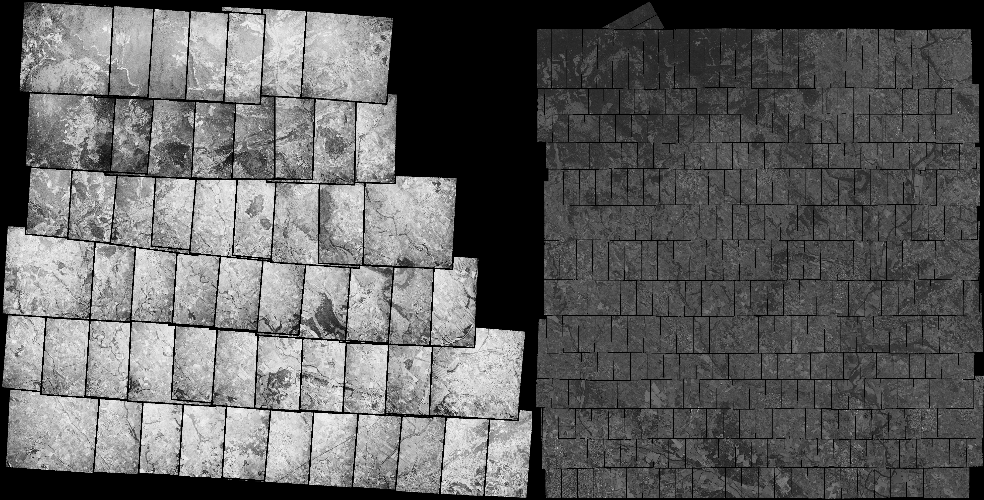
\includegraphics[width=5.1cm]{images/Chapitre3/Pseudo-Ortho-MEC-Malt_Tapas_1971_Ortho-MEC-Malt_2015.png}
			\end{minipage}%
		}
		\subfigure[Number of recovered matches(\textit{ImgPairs})]{
			\begin{minipage}[t]{0.48\linewidth}
				\centering
				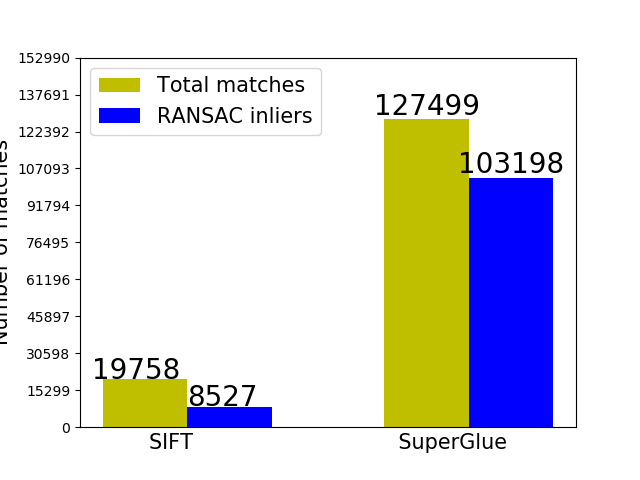
\includegraphics[width=3.5cm,trim=0 20 0 38,clip]{images/Chapitre3/PlotCurves_Pseudo-Ortho-MEC-Malt_Tapas_1971_Ortho-MEC-Malt_2015.png}
			\end{minipage}%
		}
		\subfigure[$SIFT_{ImgPairs}^{RANSAC Inliers}$]{
			\begin{minipage}[t]{0.48\linewidth}
				\centering
				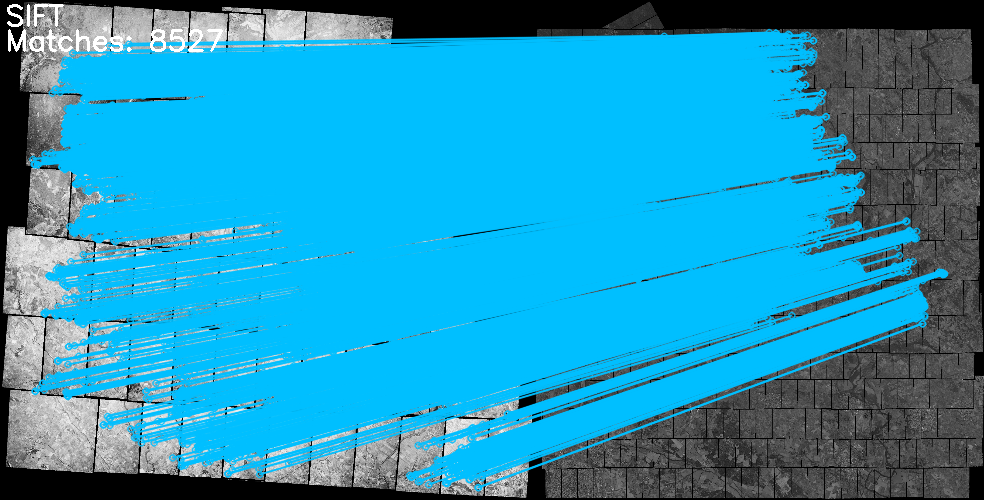
\includegraphics[width=5.2cm]{images/Chapitre3/Pseudo-Homol-SIFT2Step_1971-2015-Rough-2DRANSAC-GlobalR3D-PileImg_Ortho-MEC-Malt_Tapas_1971_Ortho-MEC-Malt_2015.png}
			\end{minipage}%
		}
		\subfigure[$SuperGlue_{ImgPairs}^{RANSAC Inliers}$]{
			\begin{minipage}[t]{0.48\linewidth}
				\centering
				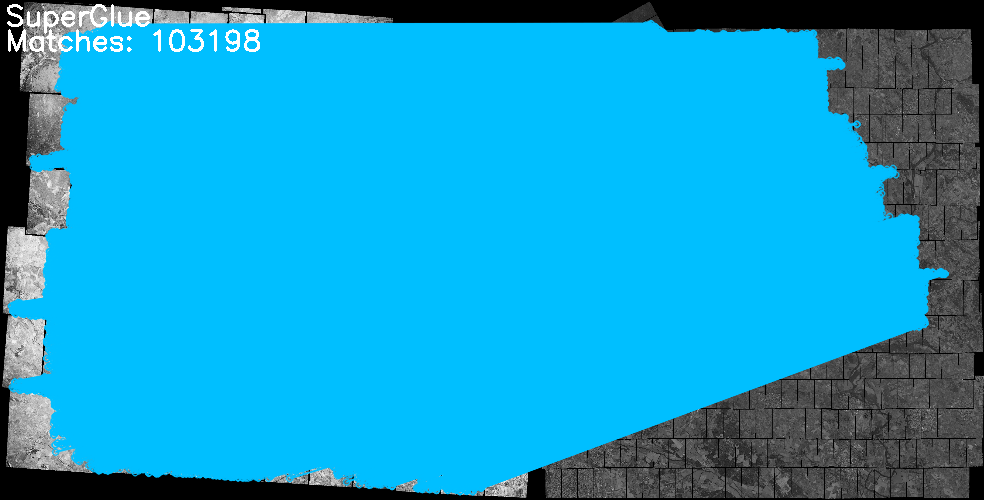
\includegraphics[width=5.2cm]{images/Chapitre3/Pseudo-Homol-SuperGlue_1971-2015-GlobalR3D-PileImg_Ortho-MEC-Malt_Tapas_1971_Ortho-MEC-Malt_2015.png}
			\end{minipage}%
		}
		%        \caption{Result of matching image pairs (i.e. \textit{ImgPairs}) of Pezenas 1971 and 2015. (a) Image pairs to be matched, with red rectangles indicating the common zone. (b) Numbers of total matches and RANSAC inliers of both SIFT and SuperGlue. (c) Visualization of RANSAC inliers based on SIFT. (d) Visualization of RANSAC inliers based on SuperGlue.}
		%        \label{MatchVizPezenas1971ImgPairs}
		%    \end{center}
		%\end{figure*} 
		%
		%\begin{figure*}[htbp]
		%    \begin{center}
		\subfigure[Orthophotos]{
			\begin{minipage}[t]{0.48\linewidth}
				\centering
				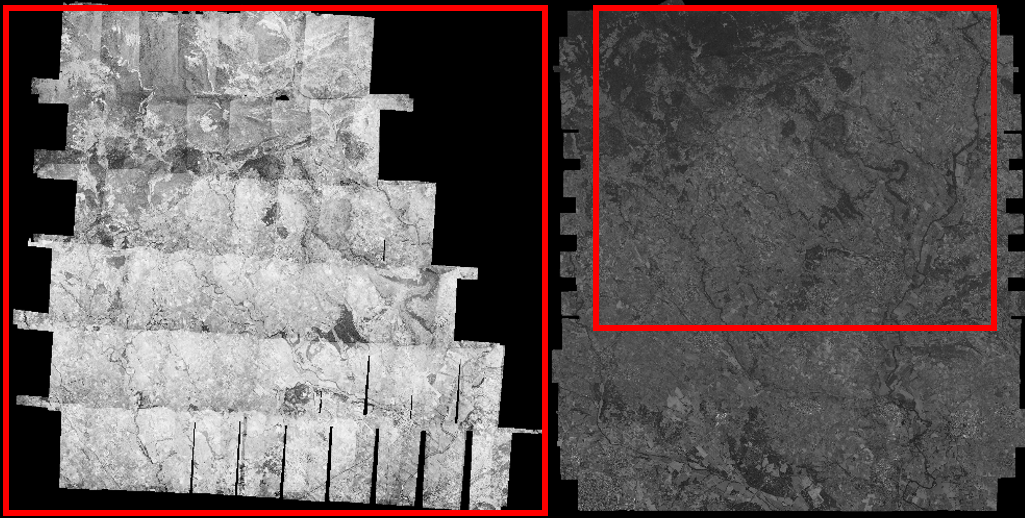
\includegraphics[width=5.1cm]{images/Chapitre3/Ortho-MEC-Malt_Tapas_1971_Ortho-MEC-Malt_2015.png}
			\end{minipage}%
		}
		\subfigure[Number of recovered matches(\textit{Ortho})]{
			\begin{minipage}[t]{0.48\linewidth}
				\centering
				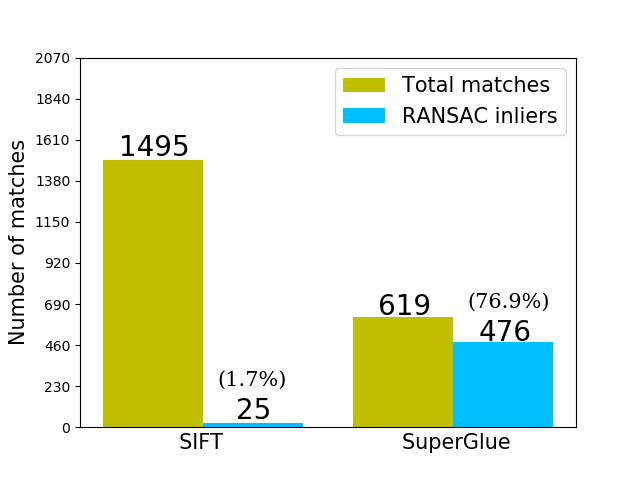
\includegraphics[width=3.5cm,trim=0 20 0 38,clip]{images/Chapitre3/PlotCurves_Ortho-MEC-Malt_Tapas_1971_Ortho-MEC-Malt_2015.png}
			\end{minipage}%
		}
		\subfigure[$SIFT_{Ortho}^{RANSAC Inliers}$]{
			\begin{minipage}[t]{0.48\linewidth}
				\centering
				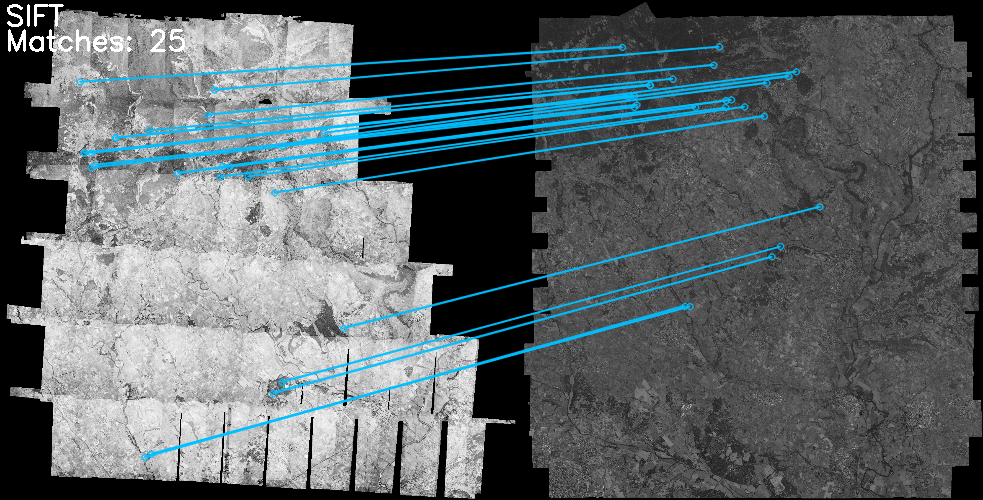
\includegraphics[width=5.2cm]{images/Chapitre3/Homol-SIFT2Step-Rough-2DRANSAC_Ortho-MEC-Malt_Tapas_1971_Ortho-MEC-Malt_2015.png}
			\end{minipage}%
		}
		\subfigure[$SuperGlue_{Ortho}^{RANSAC Inliers}$]{
			\begin{minipage}[t]{0.48\linewidth}
				\centering
				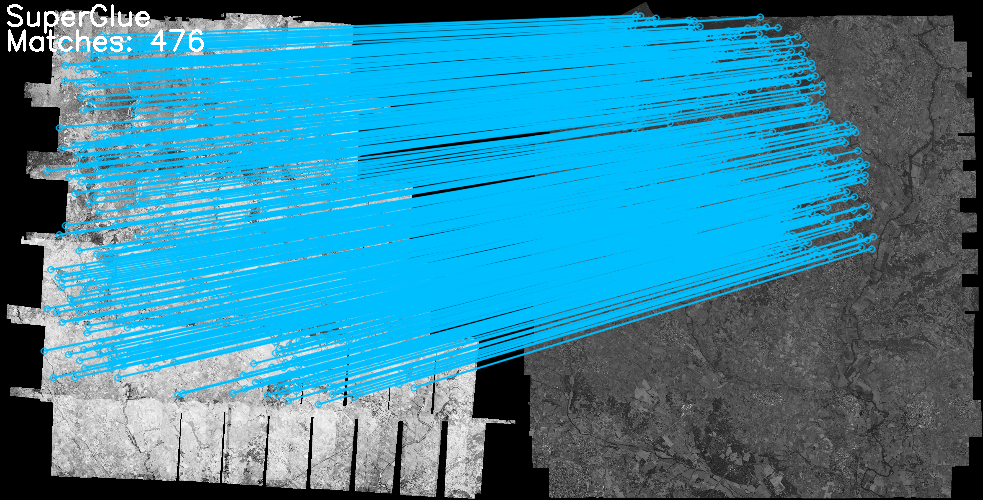
\includegraphics[width=5.2cm]{images/Chapitre3/Homol-SubPatch_R270-2DRANSAC_Ortho-MEC-Malt_Tapas_1971_Ortho-MEC-Malt_2015.png}
			\end{minipage}%
		}
		%        \caption{Result of matching orthophotos (i.e. \textit{Ortho}) of Pezenas 1971 and 2015. (a) Orthophotos to be matched, with red rectangles indicating the common zone. (b) Numbers of total matches and RANSAC inliers of both SIFT and SuperGlue. (c) Visualization of RANSAC inliers based on SIFT. (d) Visualization of RANSAC inliers based on SuperGlue.}
		%        \label{MatchVizPezenas1971Ortho}
		%    \end{center}
		%\end{figure*} 
		%
		%\begin{figure*}[htbp]
		%    \begin{center}
		\subfigure[DSMs]{
			\begin{minipage}[t]{0.48\linewidth}
				\centering
				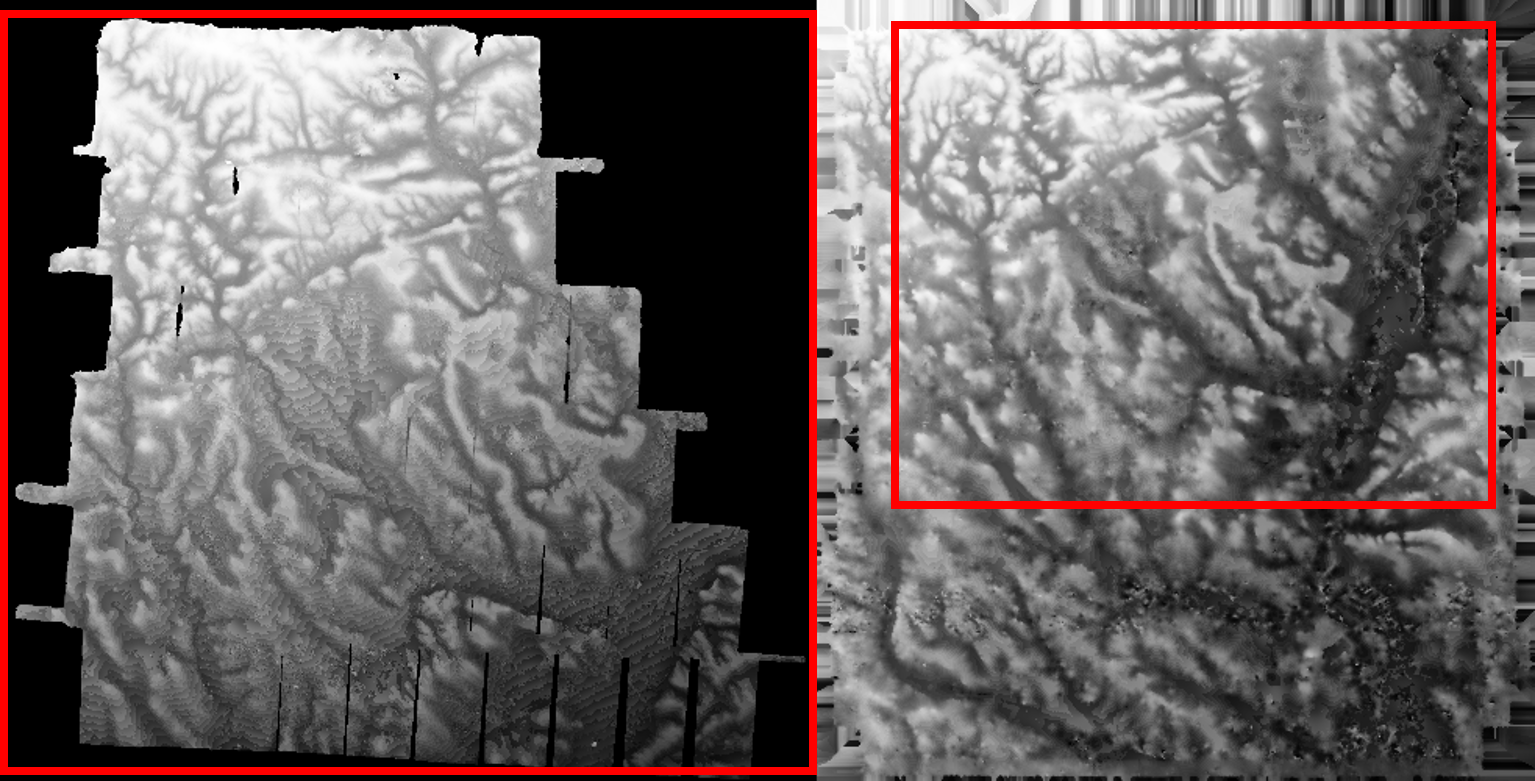
\includegraphics[width=5.1cm]{images/Chapitre3/MEC-Malt_Tapas_1971_MEC-Malt_2015.png}
			\end{minipage}%
		}
		\subfigure[Number of recovered matches(\textit{DSM})]{
			\begin{minipage}[t]{0.48\linewidth}
				\centering
				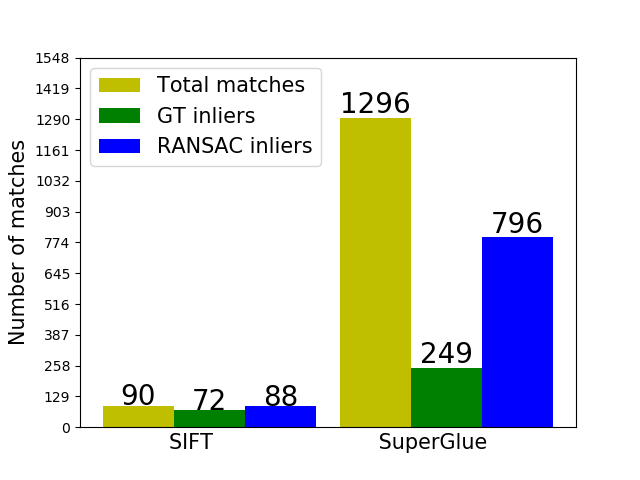
\includegraphics[width=3.5cm,trim=0 20 0 38,clip]{images/Chapitre3/PlotCurves_MEC-Malt_Tapas_1971_MEC-Malt_2015.png}
			\end{minipage}%
		}
		\subfigure[$SIFT_{DSM}^{RANSAC Inliers}$]{
			\begin{minipage}[t]{0.48\linewidth}
				\centering
				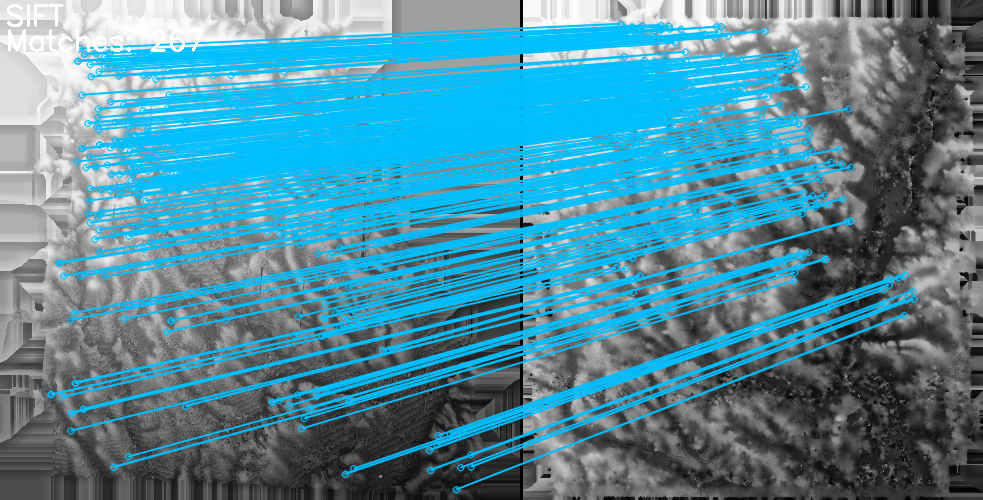
\includegraphics[width=5.2cm]{images/Chapitre3/Homol-SIFT2Step-Rough-2DRANSAC_MEC-Malt_Tapas_1971_MEC-Malt_2015.png}
			\end{minipage}%
		}
		\subfigure[$SuperGlue_{DSM}^{RANSAC Inliers}$]{
			\begin{minipage}[t]{0.48\linewidth}
				\centering
				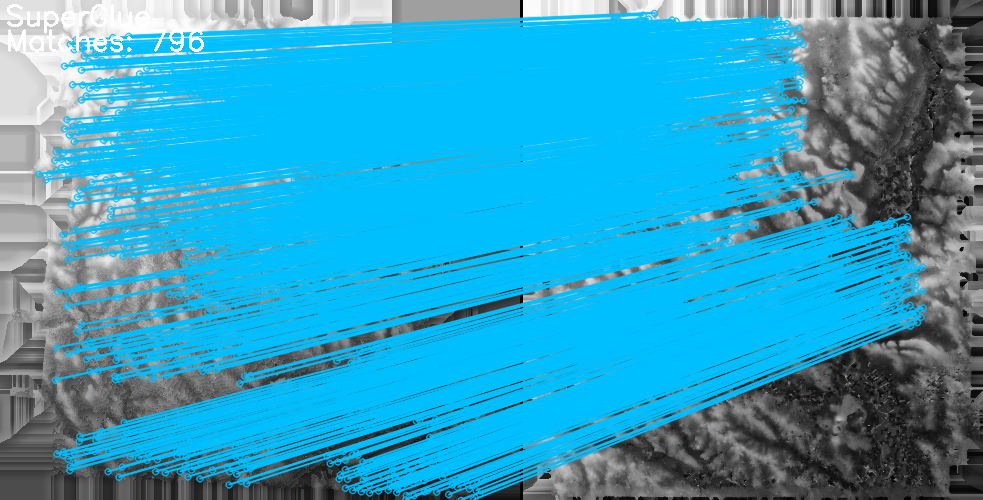
\includegraphics[width=5.2cm]{images/Chapitre3/Homol-SubPatch_R270-2DRANSAC_MEC-Malt_Tapas_1971_MEC-Malt_2015.png}
			\end{minipage}%
		}
		%\caption{Result of matching DSMs (i.e. \textit{DSM}) of Pezenas 1971 and 2015. (a) DSMs to be matched, with red rectangles indicating the common zone. (b) Numbers of total matches and RANSAC inliers of both SIFT and SuperGlue. (c) Visualization of RANSAC inliers based on SIFT. (d) Visualization of RANSAC inliers based on SuperGlue.}
		%\caption{{\small Result of \textit{ImgPairs}, \textit{Ortho} and \textit{DSM} on Pezenas 1971 and 2015. (a, e, i) image pairs/orthophotos/DSMs to be matched, with red rectangles indicating the common zone. (b, f, j) Numbers of total matches and RANSAC inliers of both SIFT and SuperGlue on methods \textit{ImgPairs}, \textit{Ortho} and \textit{DSM} individually. (c, g, k) Visualization of RANSAC inliers based on $SIFT_{ImgPairs}$, $SIFT_{Ortho}$ and $SIFT_{DSM}$. (d, h, l) Visualization of RANSAC inliers based on $SuperGlue_{ImgPairs}$, $SuperGlue_{Ortho}$ and $SuperGlue_{DSM}$.}}
		\caption{{\scriptsize Result of \textit{ImgPairs} (a-d), \textit{Ortho} (e-h) and \textit{DSM} (i-l) on matching \textbf{Pezenas 1971 and 2015}. (a, e, i) Image pairs/orthophotos/DSMs to be matched, with red rectangles indicating the common zone. (b, f, j) Numbers of total matches and RANSAC inliers of both SIFT and SuperGlue on methods \textit{ImgPairs}, \textit{Ortho} and \textit{DSM} individually. (c, g, k) Visualization of RANSAC inliers based on $SIFT_{ImgPairs}$, $SIFT_{Ortho}$ and $SIFT_{DSM}$. (d, h, l) Visualization of RANSAC inliers based on $SuperGlue_{ImgPairs}$, $SuperGlue_{Ortho}$ and $SuperGlue_{DSM}$.}}        
		\label{MatchVizPezenas1971DSM}
	\end{center}
\end{figure*} 



\begin{figure*}[htbp]
	\begin{center}
		\subfigure[Image pairs (27$\times$382 pairs)]{
			\begin{minipage}[t]{0.48\linewidth}
				\centering
				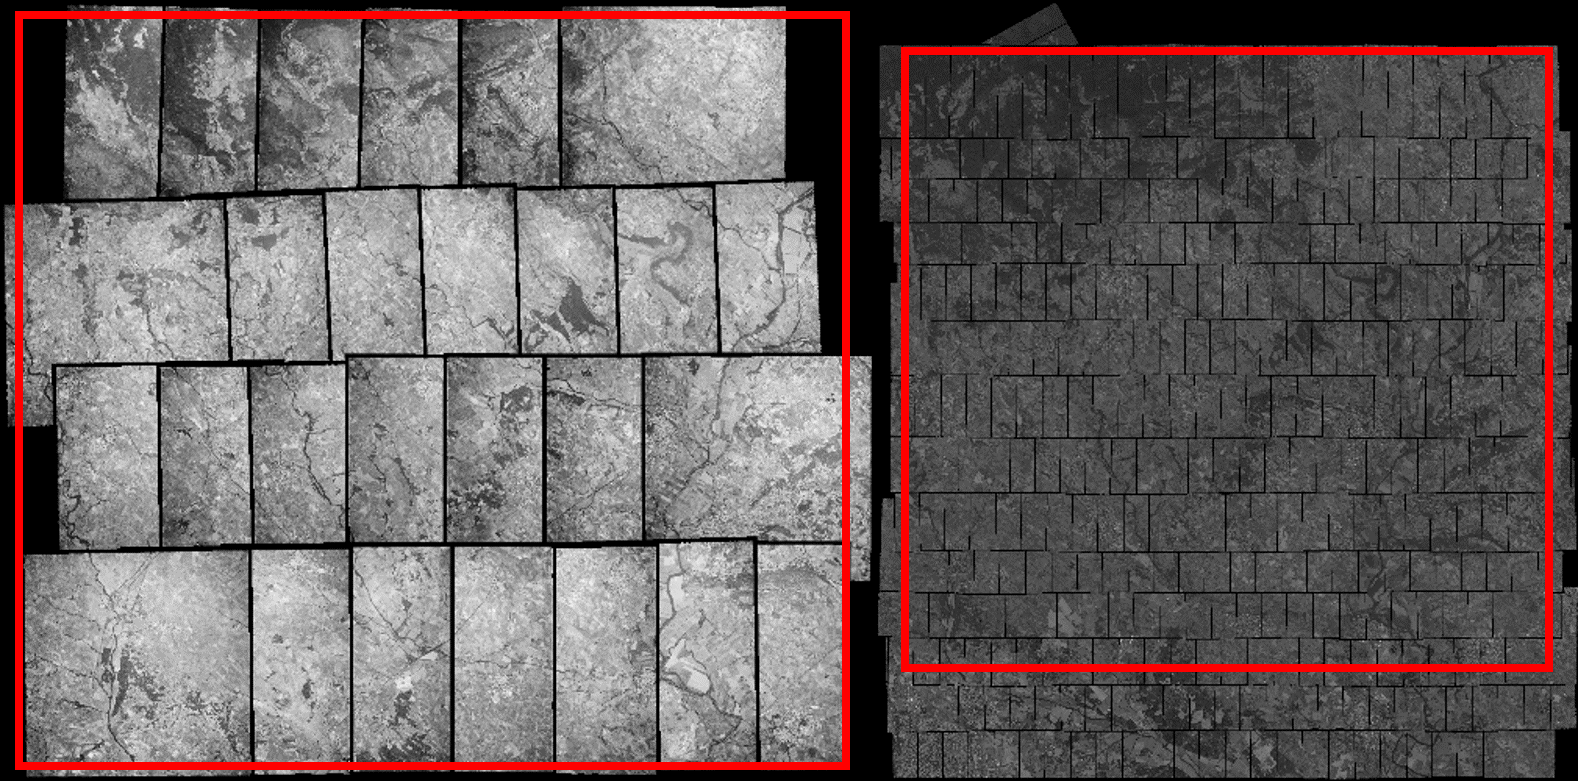
\includegraphics[width=5.1cm]{images/Chapitre3/Pseudo-Ortho-MEC-Malt_Tapas_1981_Ortho-MEC-Malt_2015.png}
			\end{minipage}%
		}
		\subfigure[Number of recovered matches(\textit{ImgPairs})]{
			\begin{minipage}[t]{0.48\linewidth}
				\centering
				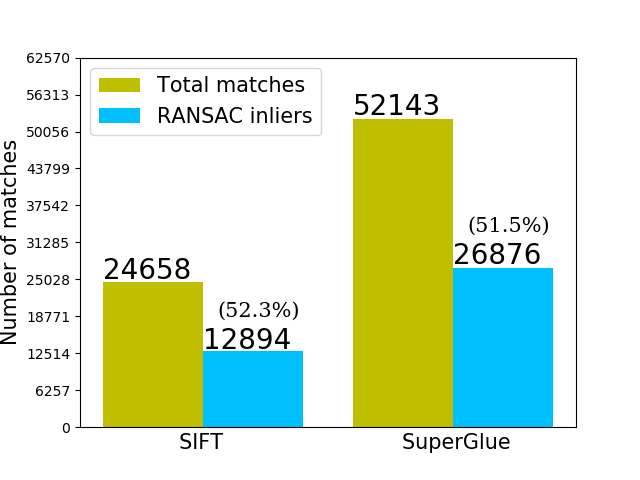
\includegraphics[width=3.5cm,trim=0 20 0 38,clip]{images/Chapitre3/PlotCurves_Pseudo-Ortho-MEC-Malt_Tapas_1981_Ortho-MEC-Malt_2015.png}
			\end{minipage}%
		}
		\subfigure[$SIFT_{ImgPairs}^{RANSAC Inliers}$]{
			\begin{minipage}[t]{0.48\linewidth}
				\centering
				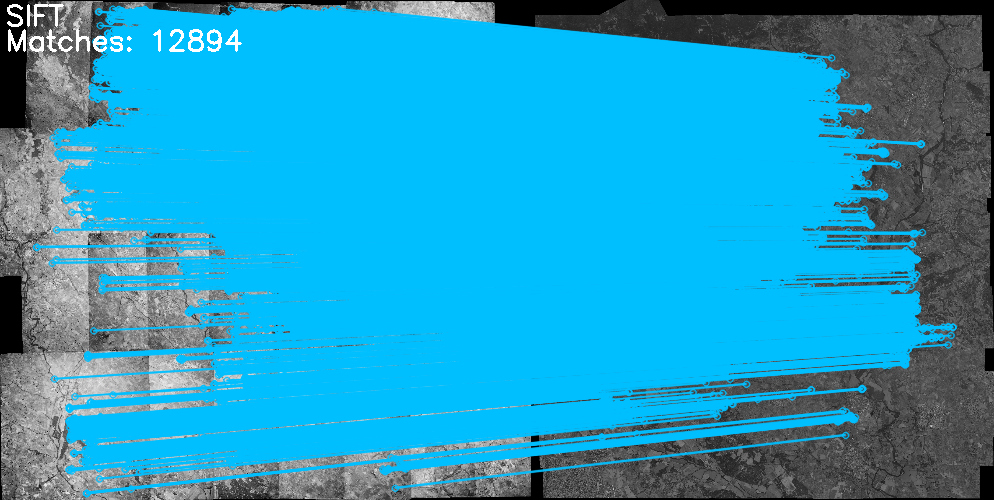
\includegraphics[width=5.2cm]{images/Chapitre3/Pseudo-Homol-SIFT2Step_1981-2015-Rough-2DRANSAC-GlobalR3D-PileImg_Ortho-MEC-Malt_Tapas_1981_Ortho-MEC-Malt_2015.png}
			\end{minipage}%
		}
		\subfigure[$SuperGlue_{ImgPairs}^{RANSAC Inliers}$]{
			\begin{minipage}[t]{0.48\linewidth}
				\centering
				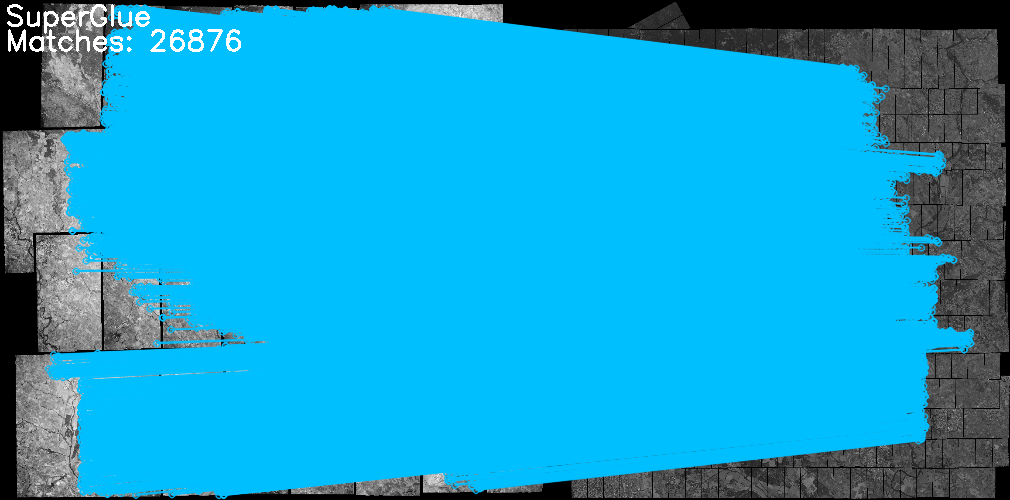
\includegraphics[width=5.2cm]{images/Chapitre3/Pseudo-Homol-SuperGlue_1981-2015-GlobalR3D-PileImg_Ortho-MEC-Malt_Tapas_1981_Ortho-MEC-Malt_2015.png}
			\end{minipage}%
		}
		%        \caption{Result of matching image pairs (i.e. \textit{ImgPairs}) of Pezenas 1981 and 2015. (a) Image pairs to be matched, with red rectangles indicating the common zone. (b) Numbers of total matches and RANSAC inliers of both SIFT and SuperGlue. (c) Visualization of RANSAC inliers based on SIFT. (d) Visualization of RANSAC inliers based on SuperGlue.}
		%        \label{MatchVizPezenas1981ImgPairs}
		%    \end{center}
		%\end{figure*} 
		%
		%\begin{figure*}[htbp]
		%    \begin{center}
		\subfigure[Orthophotos]{
			\begin{minipage}[t]{0.48\linewidth}
				\centering
				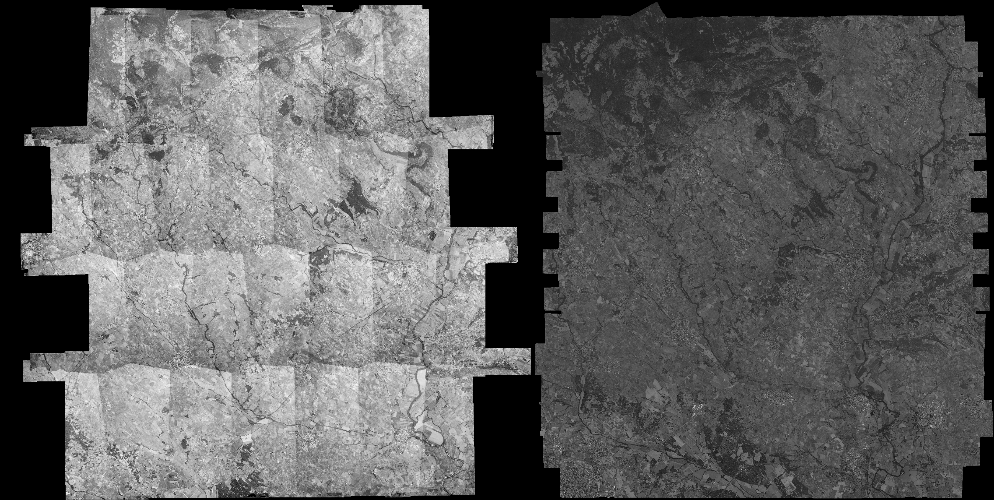
\includegraphics[width=5.1cm]{images/Chapitre3/Ortho-MEC-Malt_Tapas_1981_Ortho-MEC-Malt_2015.png}
			\end{minipage}%
		}
		\subfigure[Number of recovered matches(\textit{Ortho})]{
			\begin{minipage}[t]{0.48\linewidth}
				\centering
				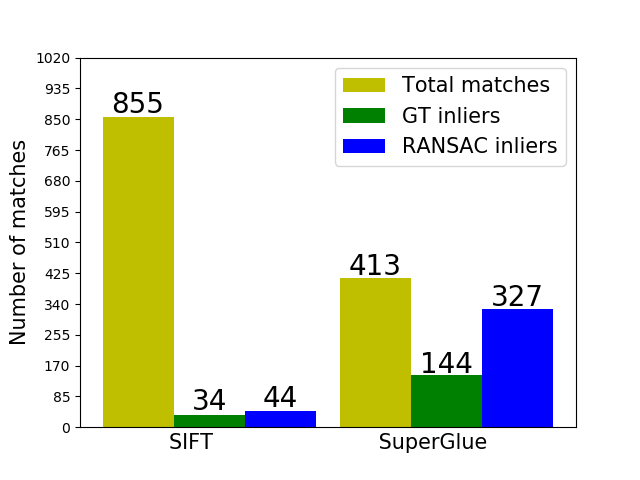
\includegraphics[width=3.5cm,trim=0 20 0 38,clip]{images/Chapitre3/PlotCurves_Ortho-MEC-Malt_Tapas_1981_Ortho-MEC-Malt_2015.png}
			\end{minipage}%
		}
		\subfigure[$SIFT_{Ortho}^{RANSAC Inliers}$]{
			\begin{minipage}[t]{0.48\linewidth}
				\centering
				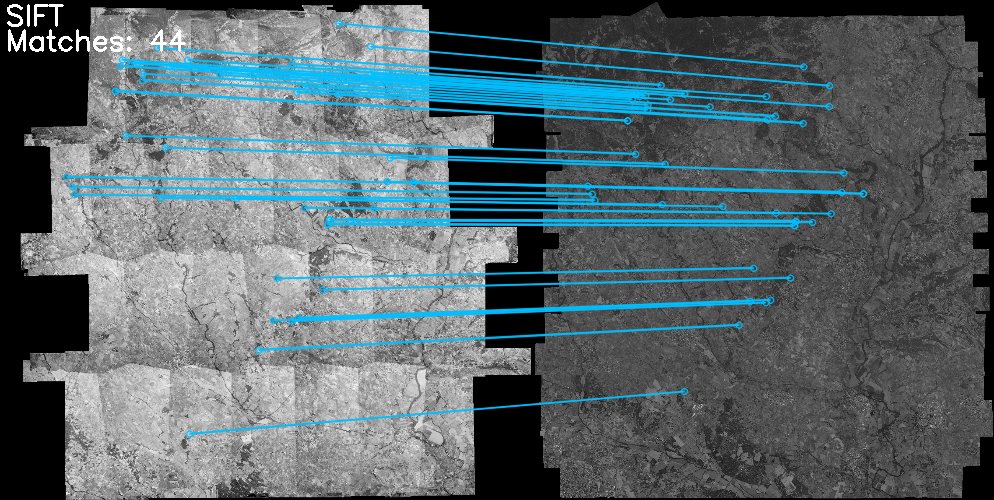
\includegraphics[width=5.2cm]{images/Chapitre3/Homol-SIFT2Step-Rough-2DRANSAC_Ortho-MEC-Malt_Tapas_1981_Ortho-MEC-Malt_2015.png}
			\end{minipage}%
		}
		\subfigure[$SuperGlue_{Ortho}^{RANSAC Inliers}$]{
			\begin{minipage}[t]{0.48\linewidth}
				\centering
				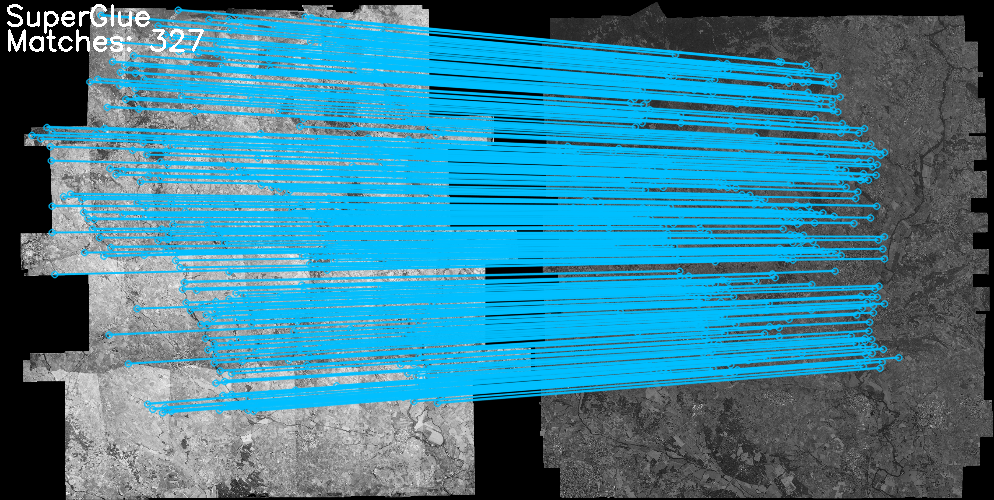
\includegraphics[width=5.2cm]{images/Chapitre3/Homol-SubPatch_R90-2DRANSAC_Ortho-MEC-Malt_Tapas_1981_Ortho-MEC-Malt_2015.png}
			\end{minipage}%
		}
		%        \caption{Result of matching orthophotos (i.e. \textit{Ortho}) of Pezenas 1981 and 2015. (a) Orthophotos to be matched, with red rectangles indicating the common zone. (b) Numbers of total matches and RANSAC inliers of both SIFT and SuperGlue. (c) Visualization of RANSAC inliers based on SIFT. (d) Visualization of RANSAC inliers based on SuperGlue.}
		%        \label{MatchVizPezenas1981Ortho}
		%    \end{center}
		%\end{figure*} 
		%
		%\begin{figure*}[htbp]
		%    \begin{center}
		\subfigure[DSMs]{
			\begin{minipage}[t]{0.48\linewidth}
				\centering
				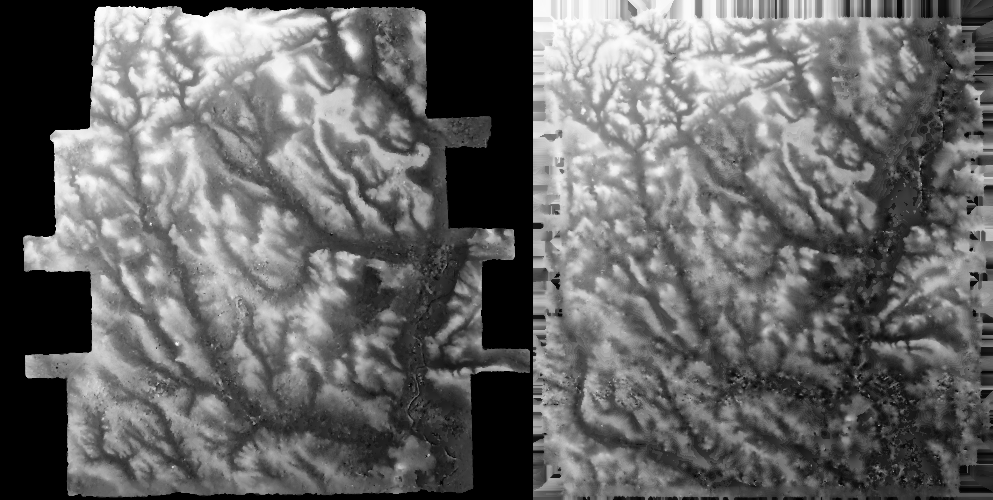
\includegraphics[width=5.1cm]{images/Chapitre3/MEC-Malt_Tapas_1981_MEC-Malt_2015.png}
			\end{minipage}%
		}
		\subfigure[Number of recovered matches(\textit{DSM})]{
			\begin{minipage}[t]{0.48\linewidth}
				\centering
				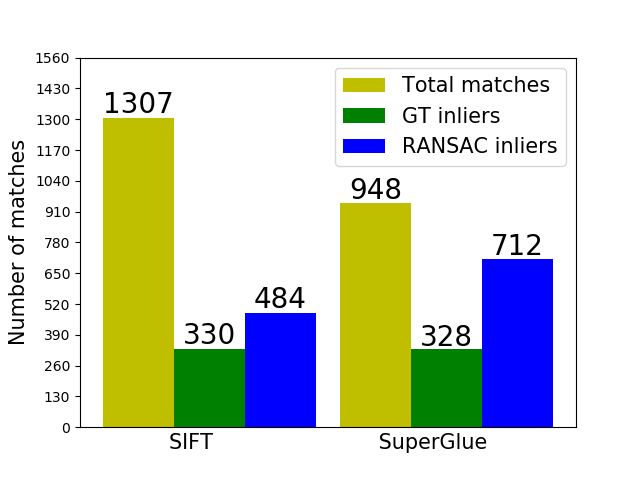
\includegraphics[width=3.5cm,trim=0 20 0 38,clip]{images/Chapitre3/PlotCurves_MEC-Malt_Tapas_1981_MEC-Malt_2015.png}
			\end{minipage}%
		}
		\subfigure[$SIFT_{DSM}^{RANSAC Inliers}$]{
			\begin{minipage}[t]{0.48\linewidth}
				\centering
				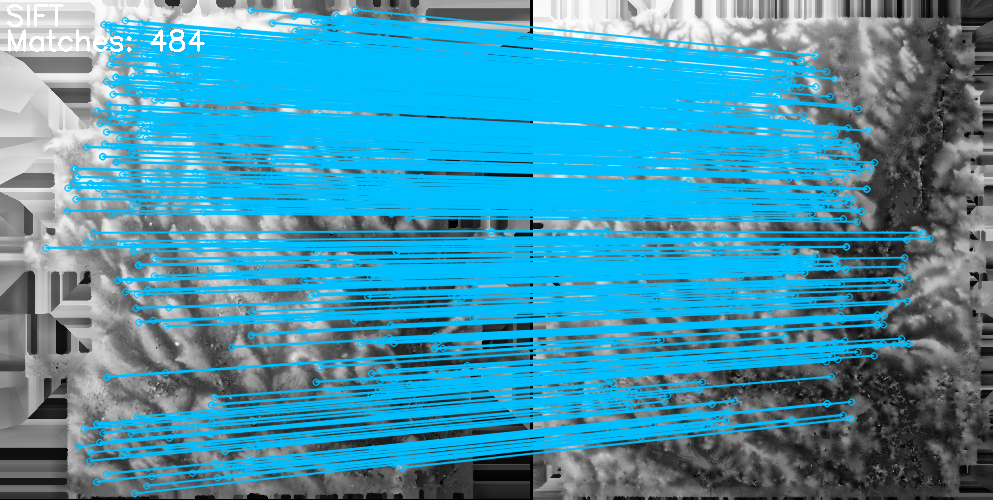
\includegraphics[width=5.2cm]{images/Chapitre3/Homol-SIFT2Step-Rough-2DRANSAC_MEC-Malt_Tapas_1981_MEC-Malt_2015.png}
			\end{minipage}%
		}
		\subfigure[$SuperGlue_{DSM}^{RANSAC Inliers}$]{
			\begin{minipage}[t]{0.48\linewidth}
				\centering
				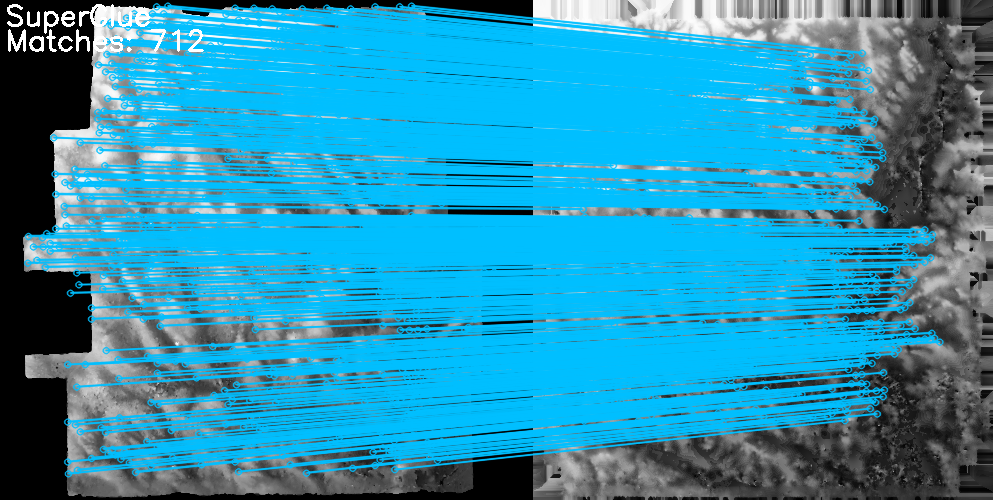
\includegraphics[width=5.2cm]{images/Chapitre3/Homol-SubPatch_R90-2DRANSAC_MEC-Malt_Tapas_1981_MEC-Malt_2015.png}
			\end{minipage}%
		}
		%\caption{Result of matching DSMs (i.e. \textit{DSM}) of Pezenas 1981 and 2015. (a) DSMs to be matched, with red rectangles indicating the common zone. (b) Numbers of total matches and RANSAC inliers of both SIFT and SuperGlue. (c) Visualization of RANSAC inliers based on SIFT. (d) Visualization of RANSAC inliers based on SuperGlue.}
		%\caption{{\small Result of \textit{ImgPairs}, \textit{Ortho} and \textit{DSM} on Pezenas 1981 and 2015. (a, e, i) image pairs/orthophotos/DSMs to be matched, with red rectangles indicating the common zone. (b, f, j) Numbers of total matches and RANSAC inliers of both SIFT and SuperGlue on methods \textit{ImgPairs}, \textit{Ortho} and \textit{DSM} individually. (c, g, k) Visualization of RANSAC inliers based on $SIFT_{ImgPairs}$, $SIFT_{Ortho}$ and $SIFT_{DSM}$. (d, h, l) Visualization of RANSAC inliers based on $SuperGlue_{ImgPairs}$, $SuperGlue_{Ortho}$ and $SuperGlue_{DSM}$.}}
		\caption{{\scriptsize Result of \textit{ImgPairs} (a-d), \textit{Ortho} (e-h) and \textit{DSM} (i-l) on matching \textbf{Pezenas 1981 and 2015}. (a, e, i) Image pairs/orthophotos/DSMs to be matched, with red rectangles indicating the common zone. (b, f, j) Numbers of total matches and RANSAC inliers of both SIFT and SuperGlue on methods \textit{ImgPairs}, \textit{Ortho} and \textit{DSM} individually. (c, g, k) Visualization of RANSAC inliers based on $SIFT_{ImgPairs}$, $SIFT_{Ortho}$ and $SIFT_{DSM}$. (d, h, l) Visualization of RANSAC inliers based on $SuperGlue_{ImgPairs}$, $SuperGlue_{Ortho}$ and $SuperGlue_{DSM}$.}}        
		\label{MatchVizPezenas1981DSM}
	\end{center}
\end{figure*} 



%%%%%%%%%%%%%%%%%%%%%%%%%%%%%%%%%%%%%%Pezenas Satellite
\begin{figure*}[htbp]
	\begin{center}
		\subfigure[Orthophotos]{
			\begin{minipage}[t]{0.48\linewidth}
				\centering
				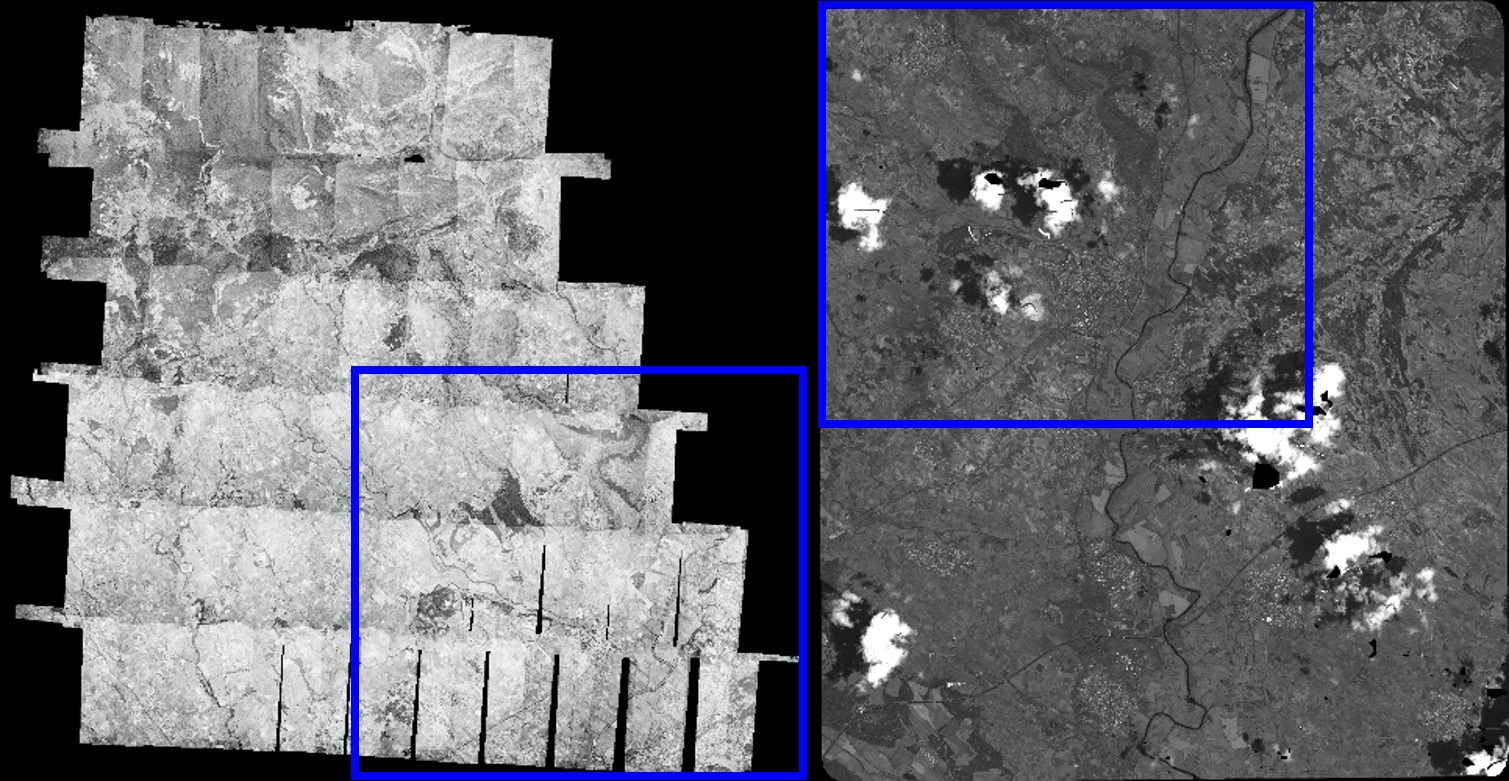
\includegraphics[width=6.8cm]{images/Chapitre3/Ortho-MEC-Malt_Tapas_1971_Ortho-MEC-Malt_Satellite.png}
			\end{minipage}%
		}
		\subfigure[Number of recovered matches(\textit{Ortho})]{
			\begin{minipage}[t]{0.48\linewidth}
				\centering
				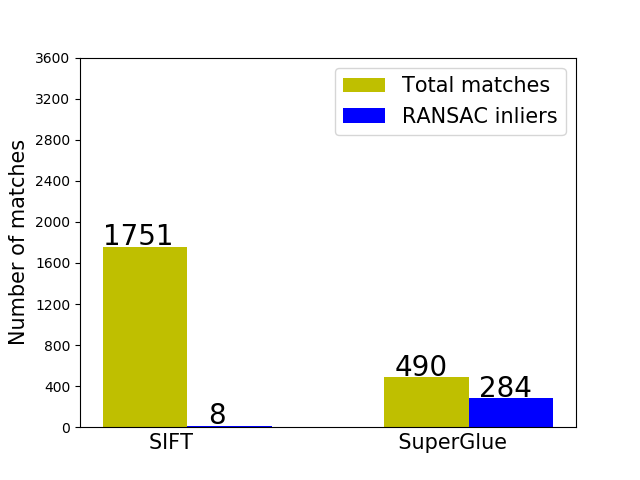
\includegraphics[width=4.9cm,trim=0 20 0 38,clip]{images/Chapitre3/PlotCurves_Ortho-MEC-Malt_Tapas_1971_Ortho-MEC-Malt_Satellite.png}
			\end{minipage}%
		}
		\subfigure[$SIFT_{Ortho}^{RANSAC Inliers}$]{
			\begin{minipage}[t]{0.48\linewidth}
				\centering
				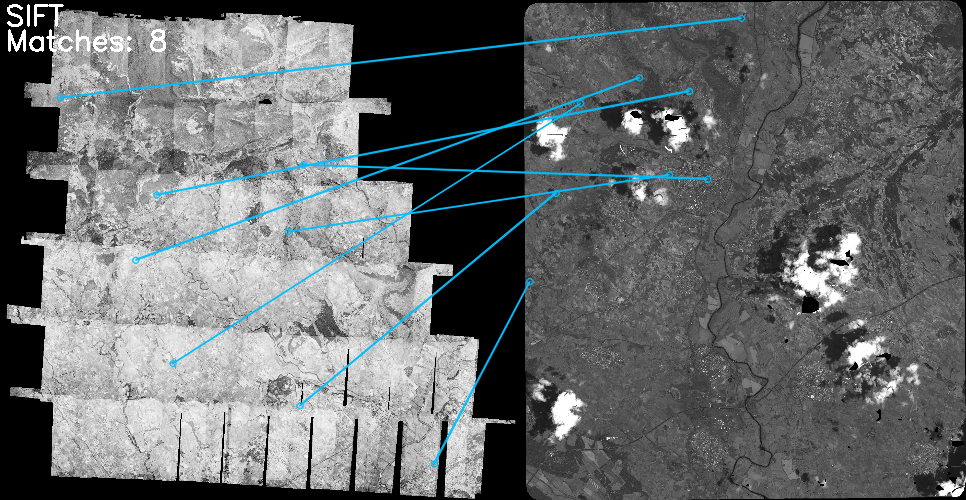
\includegraphics[width=6.8cm]{images/Chapitre3/Homol-SIFT2Step-Rough-2DRANSAC_Ortho-MEC-Malt_Tapas_1971_Ortho-MEC-Malt_Satellite.png}
			\end{minipage}%
		}
		\subfigure[$SuperGlue_{Ortho}^{RANSAC Inliers}$]{
			\begin{minipage}[t]{0.48\linewidth}
				\centering
				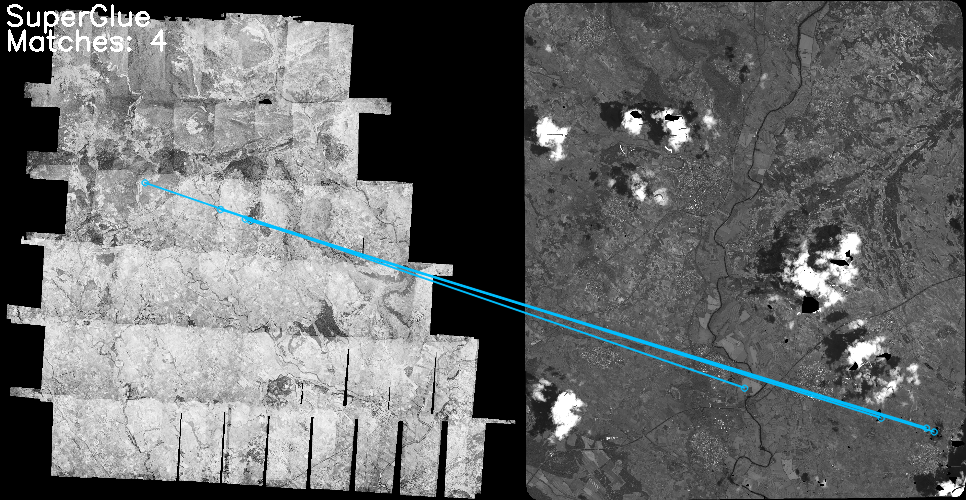
\includegraphics[width=6.8cm]{images/Chapitre3/Homol-SubPatch_R270-2DRANSAC_Ortho-MEC-Malt_Tapas_1971_Ortho-MEC-Malt_Satellite.png}
			\end{minipage}%
		}
		%        \caption{Result of matching orthophotos (i.e. \textit{Ortho}) of Pezenas 1971 and Satellite. (a) Orthophotos to be matched, with red rectangles indicating the common zone. (b) Numbers of total matches and RANSAC inliers of both SIFT and SuperGlue. (c) Visualization of RANSAC inliers based on SIFT. (d) Visualization of RANSAC inliers based on SuperGlue.}
		%        \label{MatchVizPezenas-Satellite1971Ortho}
		%    \end{center}
		%\end{figure*} 
		%
		%\begin{figure*}[htbp]
		%    \begin{center}
		\subfigure[DSMs]{
			\begin{minipage}[t]{0.48\linewidth}
				\centering
				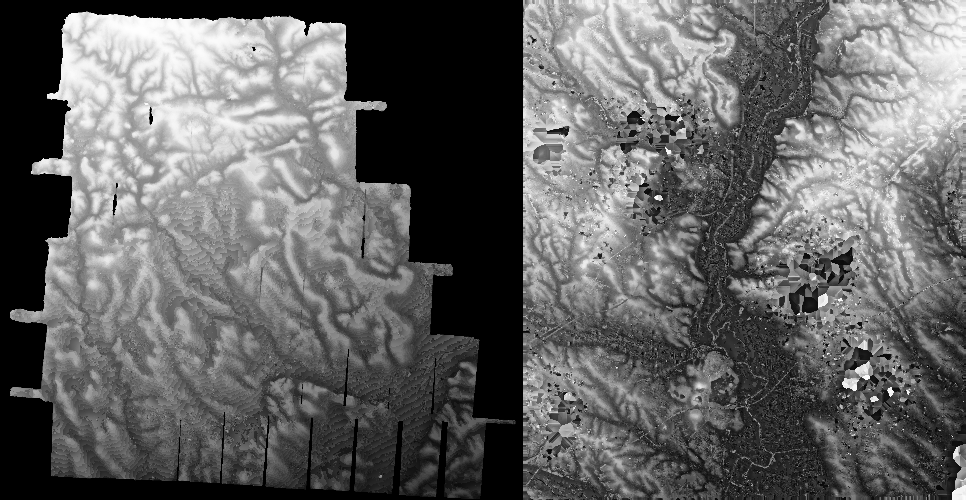
\includegraphics[width=6.8cm]{images/Chapitre3/MEC-Malt_Tapas_1971_MEC-Malt_Satellite.png}
			\end{minipage}%
		}
		\subfigure[Number of recovered matches(\textit{DSM})]{
			\begin{minipage}[t]{0.48\linewidth}
				\centering
				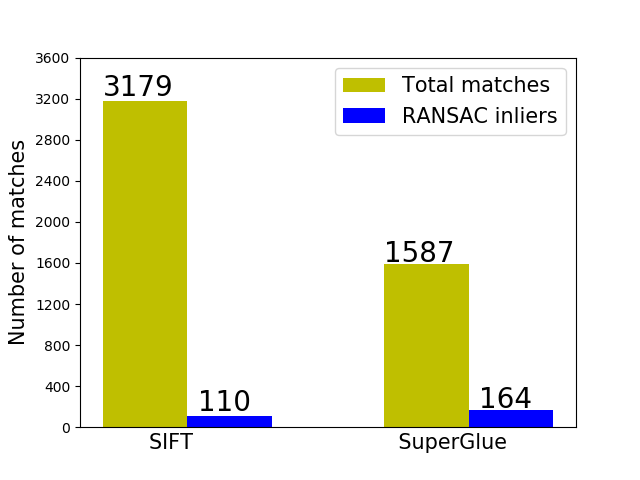
\includegraphics[width=4.9cm,trim=0 20 0 38,clip]{images/Chapitre3/PlotCurves_MEC-Malt_Tapas_1971_MEC-Malt_Satellite.png}
			\end{minipage}%
		}
		\subfigure[$SIFT_{DSM}^{RANSAC Inliers}$]{
			\begin{minipage}[t]{0.48\linewidth}
				\centering
				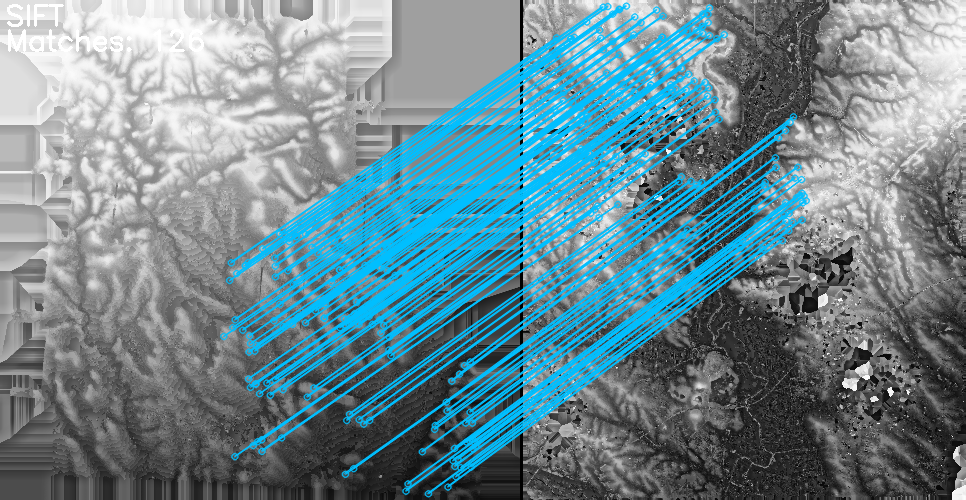
\includegraphics[width=6.8cm]{images/Chapitre3/Homol-SIFT2Step-Rough-2DRANSAC_MEC-Malt_Tapas_1971_MEC-Malt_Satellite.png}
			\end{minipage}%
		}
		\subfigure[$SuperGlue_{DSM}^{RANSAC Inliers}$]{
			\begin{minipage}[t]{0.48\linewidth}
				\centering
				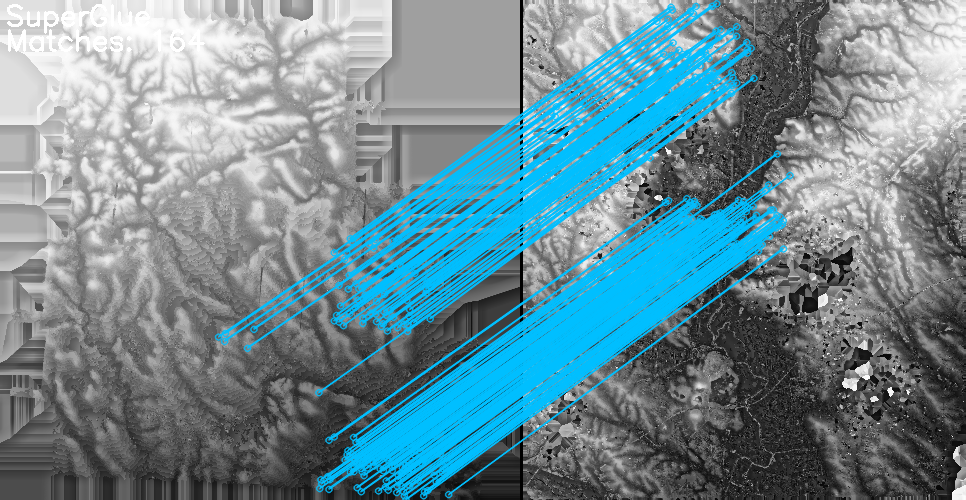
\includegraphics[width=6.8cm]{images/Chapitre3/Homol-SubPatch_R270-2DRANSAC_MEC-Malt_Tapas_1971_MEC-Malt_Satellite.png}
			\end{minipage}%
		}
		%\caption{Result of matching DSMs (i.e. \textit{DSM}) of Pezenas 1971 and Satellite. (a) DSMs to be matched, with red rectangles indicating the common zone. (b) Numbers of total matches and RANSAC inliers of both SIFT and SuperGlue. (c) Visualization of RANSAC inliers based on SIFT. (d) Visualization of RANSAC inliers based on SuperGlue.}
		%\caption{{\small Result of \textit{ImgPairs}, \textit{Ortho} and \textit{DSM} on Pezenas 1971 and Satellite. (a, e, i) image pairs/orthophotos/DSMs to be matched, with red rectangles indicating the common zone. (b, f, j) Numbers of total matches and RANSAC inliers of both SIFT and SuperGlue on methods \textit{ImgPairs}, \textit{Ortho} and \textit{DSM} individually. (c, g, k) Visualization of RANSAC inliers based on $SIFT_{ImgPairs}$, $SIFT_{Ortho}$ and $SIFT_{DSM}$. (d, h, l) Visualization of RANSAC inliers based on $SuperGlue_{ImgPairs}$, $SuperGlue_{Ortho}$ and $SuperGlue_{DSM}$.}}
		\caption{{\scriptsize Result of \textit{ImgPairs} (a-d), \textit{Ortho} (e-h) and \textit{DSM} (i-l) on matching \textbf{Pezenas 1971 and 2014 (Satellite)}. (a, e, i) Image pairs/orthophotos/DSMs to be matched, with red rectangles indicating the common zone. (b, f, j) Numbers of total matches and RANSAC inliers of both SIFT and SuperGlue on methods \textit{ImgPairs}, \textit{Ortho} and \textit{DSM} individually. (c, g, k) Visualization of RANSAC inliers based on $SIFT_{ImgPairs}$, $SIFT_{Ortho}$ and $SIFT_{DSM}$. (d, h, l) Visualization of RANSAC inliers based on $SuperGlue_{ImgPairs}$, $SuperGlue_{Ortho}$ and $SuperGlue_{DSM}$.}}        
		\label{MatchVizPezenas-Satellite1971DSM}
	\end{center}
\end{figure*} 



\begin{figure*}[htbp]
	\begin{center}
		\subfigure[Orthophotos]{
			\begin{minipage}[t]{0.48\linewidth}
				\centering
				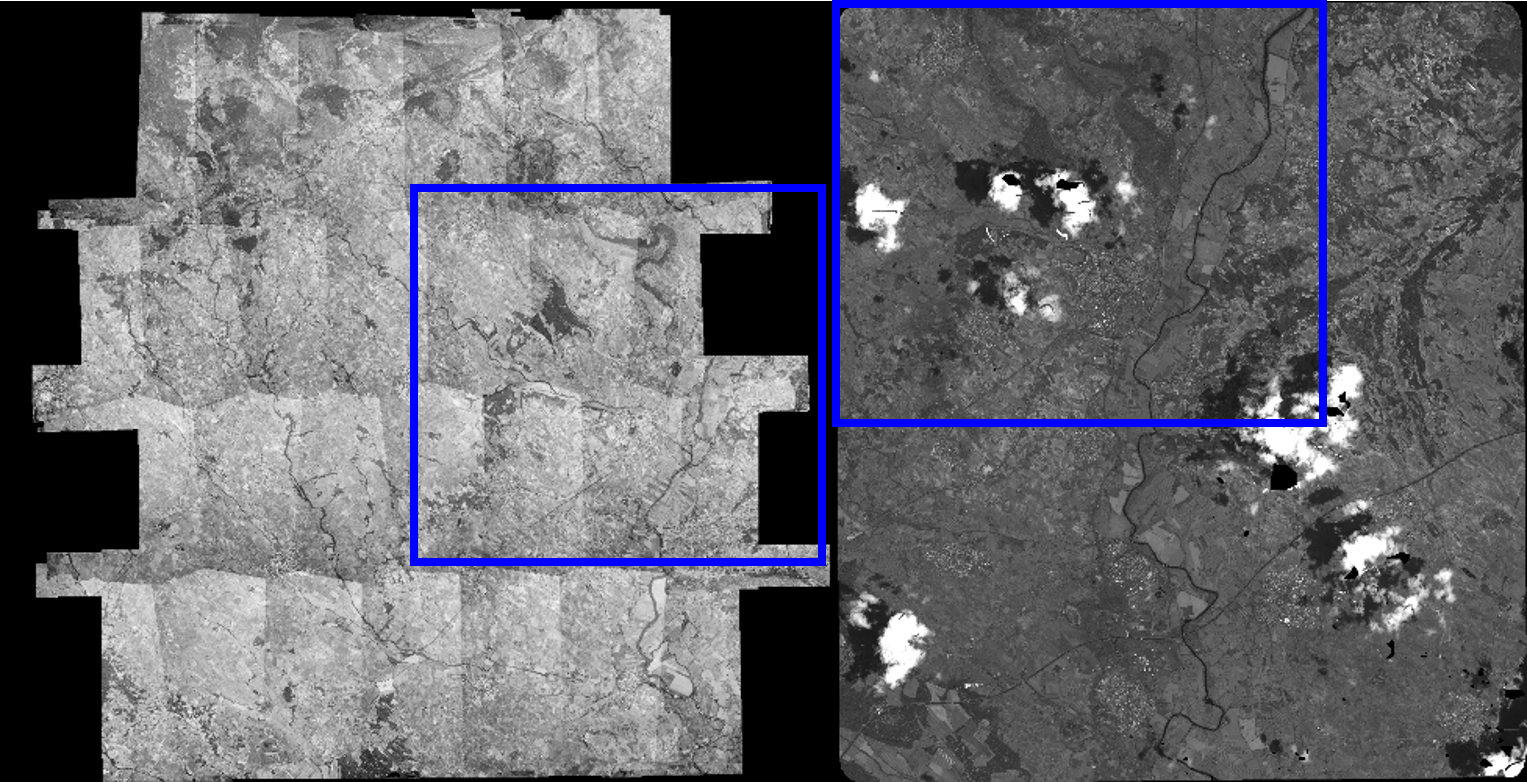
\includegraphics[width=6.8cm]{images/Chapitre3/Ortho-MEC-Malt_Tapas_1981_Ortho-MEC-Malt_Satellite.png}
			\end{minipage}%
		}
		\subfigure[Number of recovered matches(\textit{Ortho})]{
			\begin{minipage}[t]{0.48\linewidth}
				\centering
				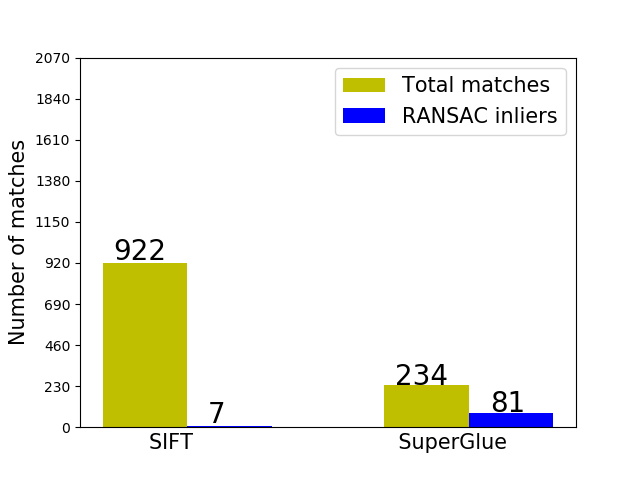
\includegraphics[width=4.9cm,trim=0 20 0 38,clip]{images/Chapitre3/PlotCurves_Ortho-MEC-Malt_Tapas_1981_Ortho-MEC-Malt_Satellite.png}
			\end{minipage}%
		}
		\subfigure[$SIFT_{Ortho}^{RANSAC Inliers}$]{
			\begin{minipage}[t]{0.48\linewidth}
				\centering
				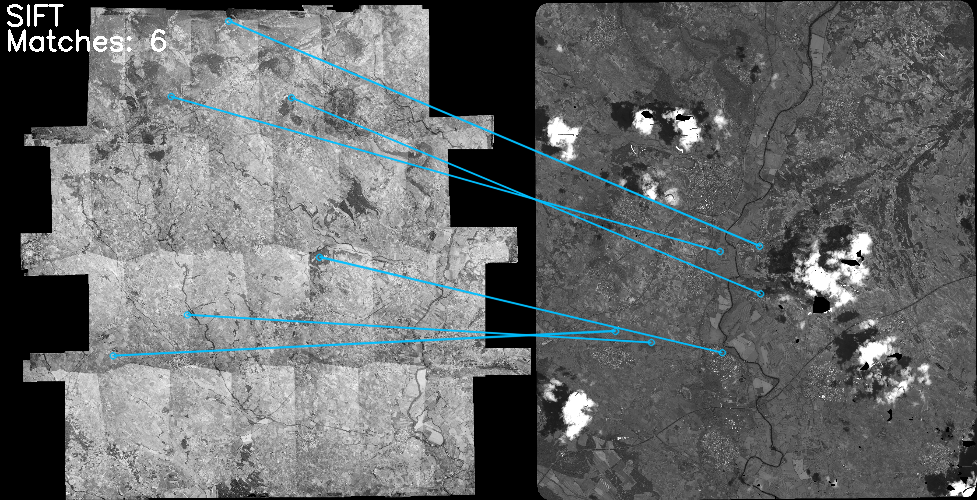
\includegraphics[width=6.8cm]{images/Chapitre3/Homol-SIFT2Step-Rough-2DRANSAC_Ortho-MEC-Malt_Tapas_1981_Ortho-MEC-Malt_Satellite.png}
			\end{minipage}%
		}
		\subfigure[$SuperGlue_{Ortho}^{RANSAC Inliers}$]{
			\begin{minipage}[t]{0.48\linewidth}
				\centering
				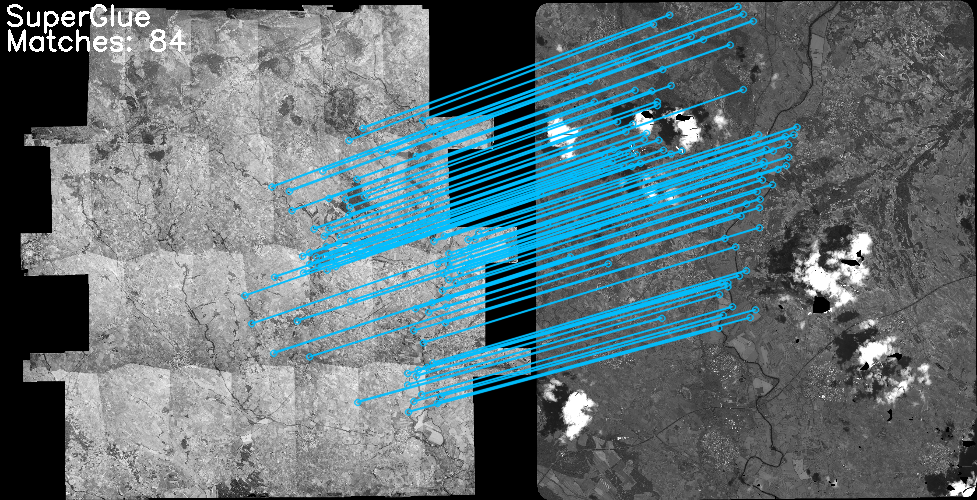
\includegraphics[width=6.8cm]{images/Chapitre3/Homol-SubPatch_R90-2DRANSAC_Ortho-MEC-Malt_Tapas_1981_Ortho-MEC-Malt_Satellite.png}
			\end{minipage}%
		}
		%        \caption{Result of matching orthophotos (i.e. \textit{Ortho}) of Pezenas 1981 and Satellite. (a) Orthophotos to be matched, with red rectangles indicating the common zone. (b) Numbers of total matches and RANSAC inliers of both SIFT and SuperGlue. (c) Visualization of RANSAC inliers based on SIFT. (d) Visualization of RANSAC inliers based on SuperGlue.}
		%        \label{MatchVizPezenas-Satellite1981Ortho}
		%    \end{center}
		%\end{figure*} 
		%
		%\begin{figure*}[htbp]
		%    \begin{center}
		\subfigure[DSMs]{
			\begin{minipage}[t]{0.48\linewidth}
				\centering
				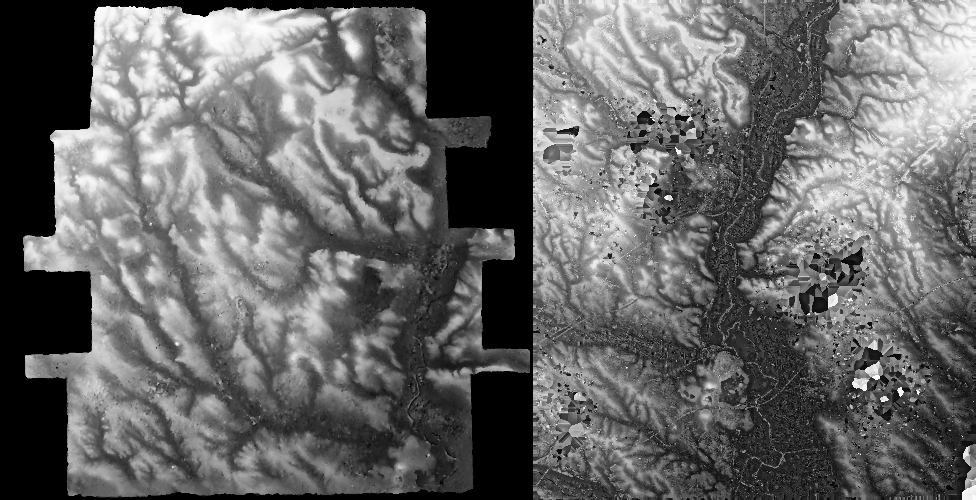
\includegraphics[width=6.8cm]{images/Chapitre3/MEC-Malt_Tapas_1981_MEC-Malt_Satellite.png}
			\end{minipage}%
		}
		\subfigure[Number of recovered matches(\textit{DSM})]{
			\begin{minipage}[t]{0.48\linewidth}
				\centering
				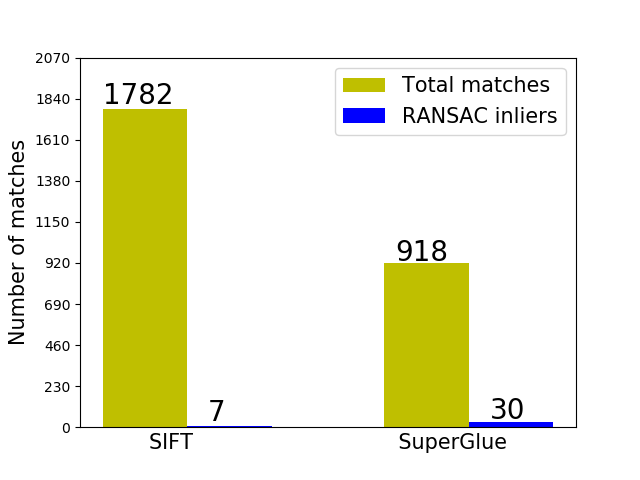
\includegraphics[width=4.9cm,trim=0 20 0 38,clip]{images/Chapitre3/PlotCurves_MEC-Malt_Tapas_1981_MEC-Malt_Satellite.png}
			\end{minipage}%
		}
		\subfigure[$SIFT_{DSM}^{RANSAC Inliers}$]{
			\begin{minipage}[t]{0.48\linewidth}
				\centering
				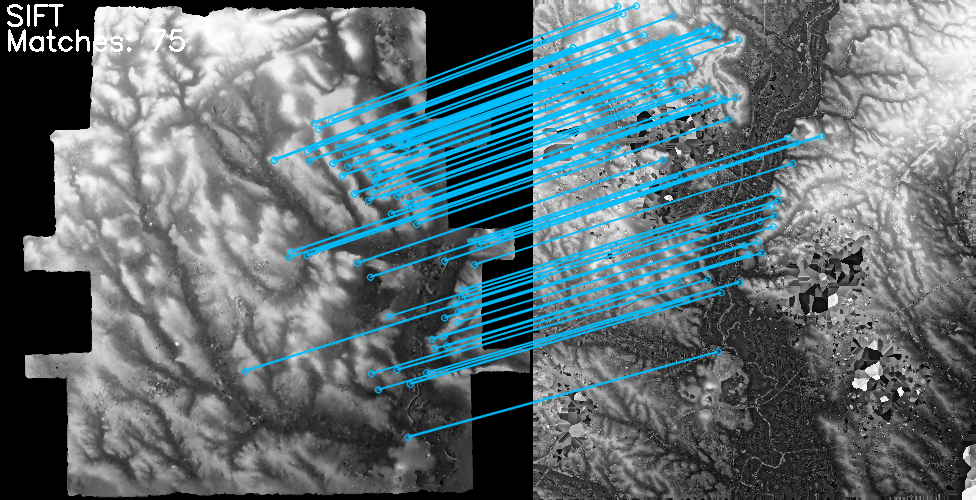
\includegraphics[width=6.8cm]{images/Chapitre3/Homol-SIFT2Step-Rough-2DRANSAC_MEC-Malt_Tapas_1981_MEC-Malt_Satellite.png}
			\end{minipage}%
		}
		\subfigure[$SuperGlue_{DSM}^{RANSAC Inliers}$]{
			\begin{minipage}[t]{0.48\linewidth}
				\centering
				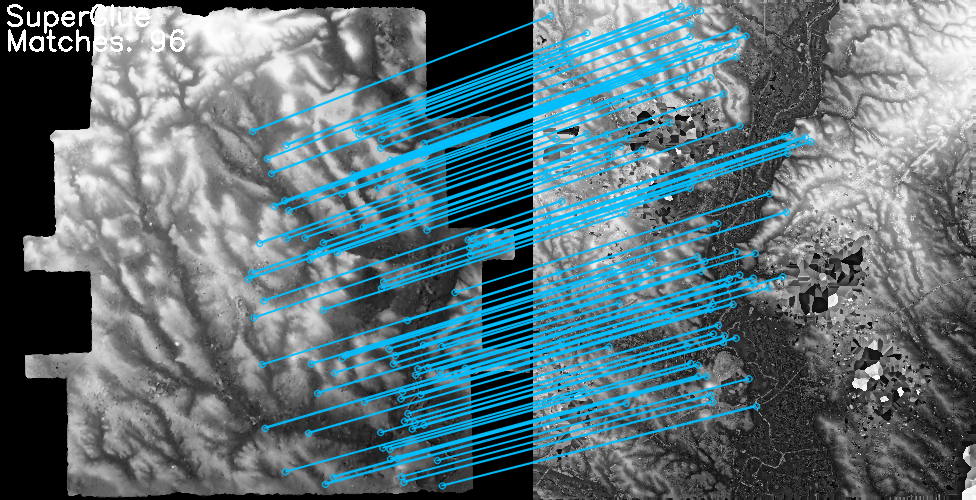
\includegraphics[width=6.8cm]{images/Chapitre3/Homol-SubPatch_R90-2DRANSAC_MEC-Malt_Tapas_1981_MEC-Malt_Satellite.png}
			\end{minipage}%
		}
		%\caption{Result of matching DSMs (i.e. \textit{DSM}) of Pezenas 1981 and Satellite. (a) DSMs to be matched, with red rectangles indicating the common zone. (b) Numbers of total matches and RANSAC inliers of both SIFT and SuperGlue. (c) Visualization of RANSAC inliers based on SIFT. (d) Visualization of RANSAC inliers based on SuperGlue.}
		%\caption{{\small Result of \textit{ImgPairs}, \textit{Ortho} and \textit{DSM} on Pezenas 1981 and Satellite. (a, e, i) image pairs/orthophotos/DSMs to be matched, with red rectangles indicating the common zone. (b, f, j) Numbers of total matches and RANSAC inliers of both SIFT and SuperGlue on methods \textit{ImgPairs}, \textit{Ortho} and \textit{DSM} individually. (c, g, k) Visualization of RANSAC inliers based on $SIFT_{ImgPairs}$, $SIFT_{Ortho}$ and $SIFT_{DSM}$. (d, h, l) Visualization of RANSAC inliers based on $SuperGlue_{ImgPairs}$, $SuperGlue_{Ortho}$ and $SuperGlue_{DSM}$.}}
		\caption{{\scriptsize Result of \textit{ImgPairs} (a-d), \textit{Ortho} (e-h) and \textit{DSM} (i-l) on matching \textbf{Pezenas 1981 and 2014 (Satellite)}. (a, e, i) Image pairs/orthophotos/DSMs to be matched, with red rectangles indicating the common zone. (b, f, j) Numbers of total matches and RANSAC inliers of both SIFT and SuperGlue on methods \textit{ImgPairs}, \textit{Ortho} and \textit{DSM} individually. (c, g, k) Visualization of RANSAC inliers based on $SIFT_{ImgPairs}$, $SIFT_{Ortho}$ and $SIFT_{DSM}$. (d, h, l) Visualization of RANSAC inliers based on $SuperGlue_{ImgPairs}$, $SuperGlue_{Ortho}$ and $SuperGlue_{DSM}$.}}        
		\label{MatchVizPezenas-Satellite1981DSM}
	\end{center}
\end{figure*} 


%%%%%%%%%%%%%%%%%%%%%%%%%%%%%%%%%%%%%%Kobe

\begin{figure*}[htbp]
	\begin{center}
		\subfigure[Image pairs (15$\times$83 pairs)]{
			\begin{minipage}[t]{0.48\linewidth}
				\centering
				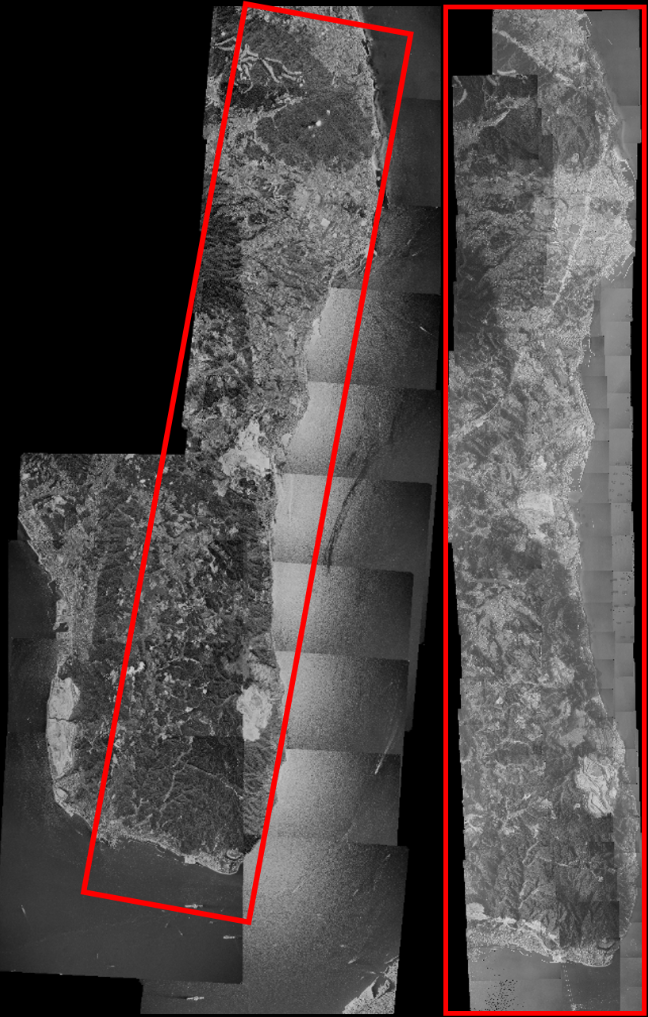
\includegraphics[width=2.3cm,angle=90]{images/Chapitre3/Pseudo-Ortho-MEC-Malt_Tapas_1991_Ortho-MEC-Malt_Tapas_1994.png}
			\end{minipage}%
		}
		\subfigure[Number of recovered matches(\textit{ImgPairs})]{
			\begin{minipage}[t]{0.48\linewidth}
				\centering
				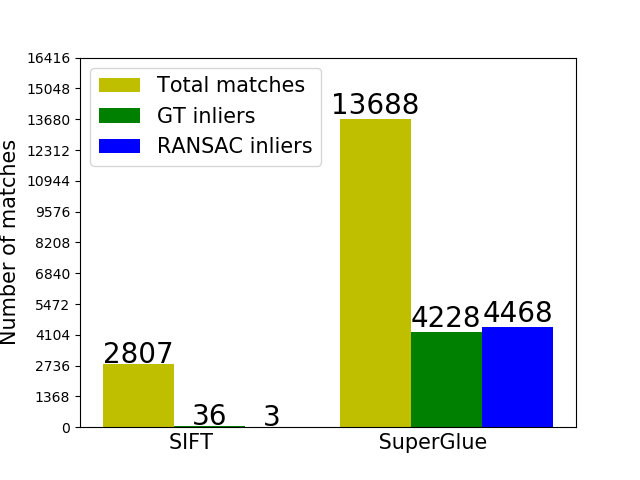
\includegraphics[width=3.5cm,trim=0 20 0 38,clip]{images/Chapitre3/PlotCurves_Pseudo-Ortho-MEC-Malt_Tapas_1991_Ortho-MEC-Malt_Tapas_1994.png}
			\end{minipage}%
		}   
		\subfigure[$SIFT_{ImgPairs}^{RANSAC Inliers}$]{
			\begin{minipage}[t]{0.48\linewidth}
				\centering
				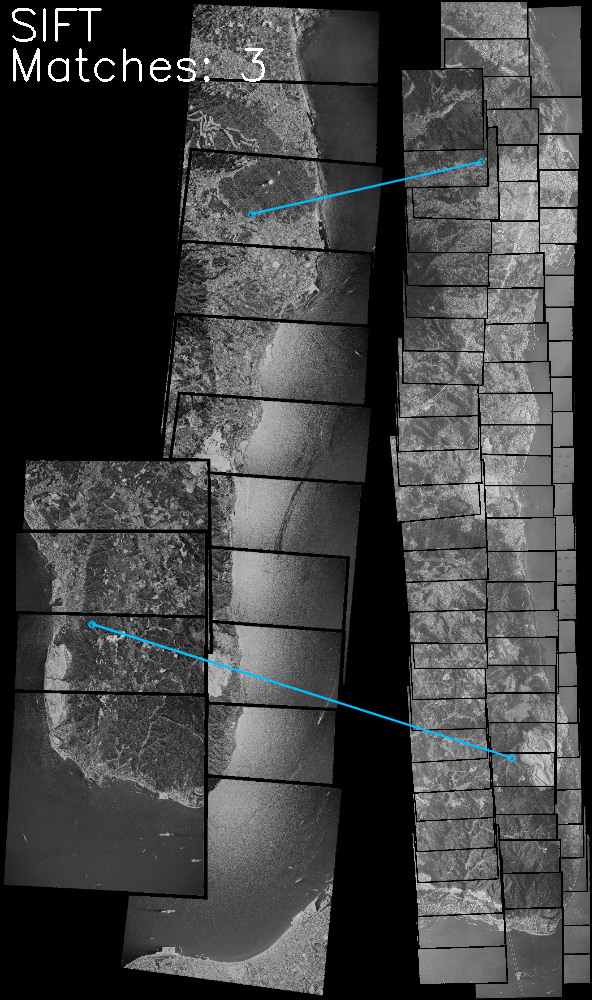
\includegraphics[width=2.6cm,angle=90]{images/Chapitre3/Pseudo-Homol-SIFT2Step_1991-1994-Rough-2DRANSAC-GlobalR3D-PileImg_Ortho-MEC-Malt_Tapas_1991_Ortho-MEC-Malt_Tapas_1994.png}
			\end{minipage}%
		}
		\subfigure[$SuperGlue_{ImgPairs}^{RANSAC Inliers}$]{
			\begin{minipage}[t]{0.48\linewidth}
				\centering
				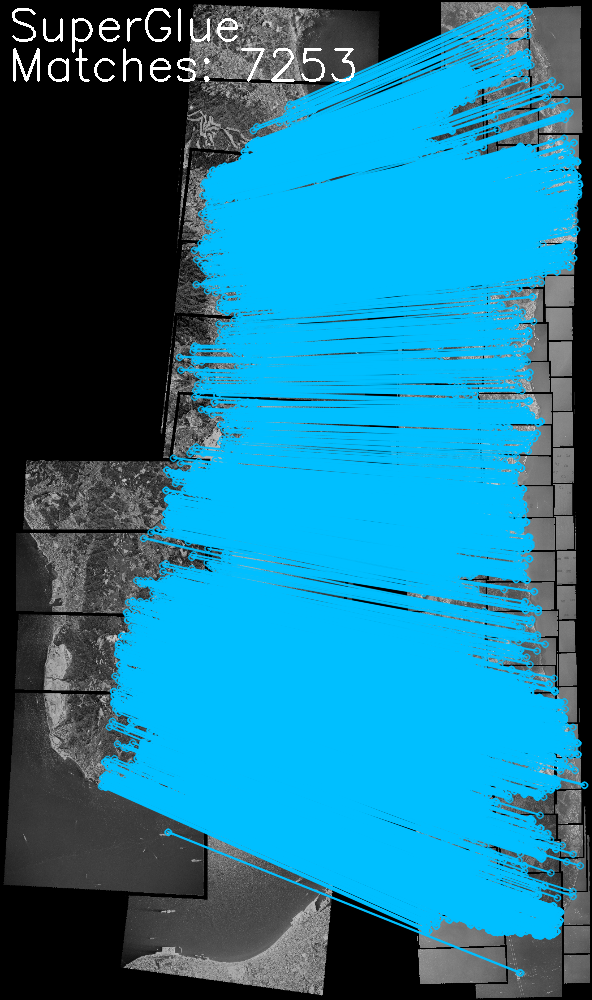
\includegraphics[width=2.6cm,angle=90]{images/Chapitre3/Pseudo-Homol-SuperGlue_1991-1994-GlobalR3D-PileImg_Ortho-MEC-Malt_Tapas_1991_Ortho-MEC-Malt_Tapas_1994.png}
			\end{minipage}%
		}
		%        \caption{Result of matching image pairs (i.e. \textit{ImgPairs}) of Kobe 1991 and 1995. (a) Image pairs to be matched, with red rectangles indicating the common zone. (b) Numbers of total matches and RANSAC inliers of both SIFT and SuperGlue. (c) Visualization of RANSAC inliers based on SIFT. (d) Visualization of RANSAC inliers based on SuperGlue.}
		%        \label{MatchVizKobe1991ImgPairs}
		%    \end{center}
		%\end{figure*} 
		%
		%\begin{figure*}[htbp]
		%    \begin{center}
		\subfigure[Orthophotos]{
			\begin{minipage}[t]{0.48\linewidth}
				\centering
				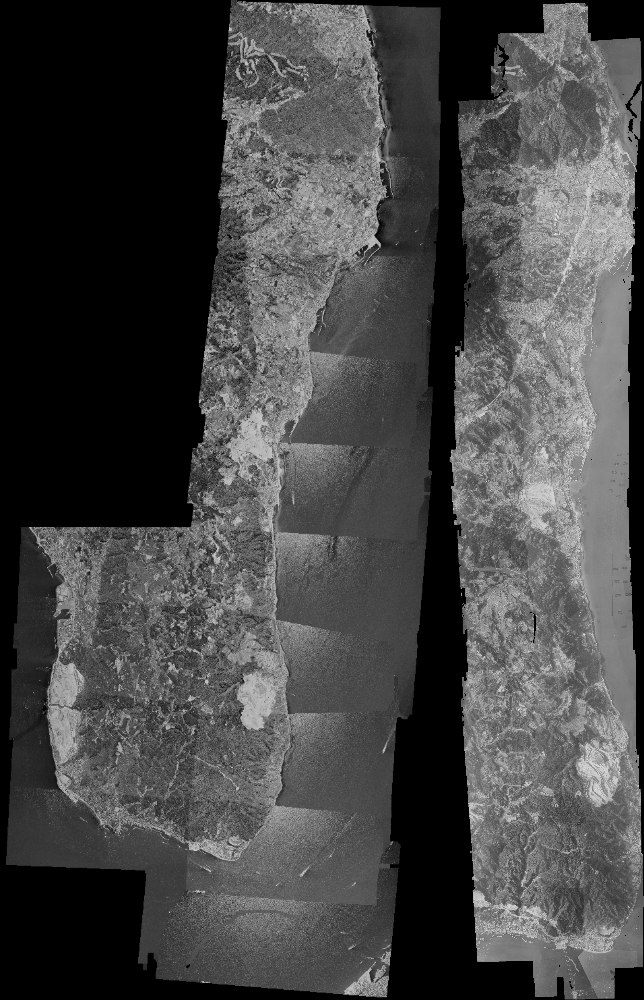
\includegraphics[width=2.3cm,angle=90]{images/Chapitre3/Ortho-MEC-Malt_Tapas_1991_Ortho-MEC-Malt_Tapas_1994.png}
			\end{minipage}%
		}
		\subfigure[Number of recovered matches(\textit{Ortho})]{
			\begin{minipage}[t]{0.48\linewidth}
				\centering
				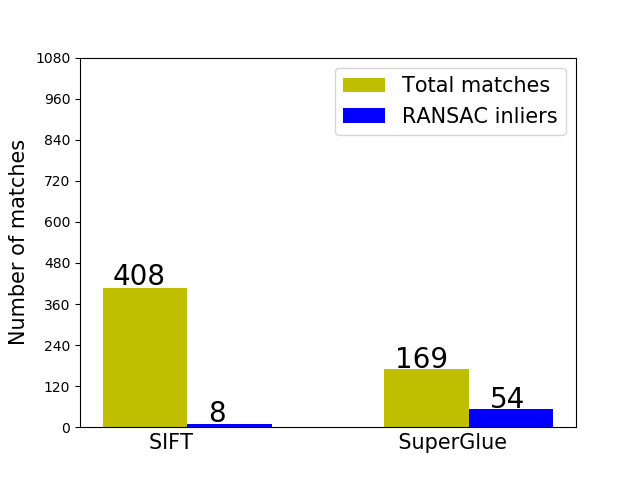
\includegraphics[width=3.5cm,trim=0 20 0 38,clip]{images/Chapitre3/PlotCurves_Ortho-MEC-Malt_Tapas_1991_Ortho-MEC-Malt_Tapas_1994.png}
			\end{minipage}%
		}   
		\subfigure[$SIFT_{Ortho}^{RANSAC Inliers}$]{
			\begin{minipage}[t]{0.48\linewidth}
				\centering
				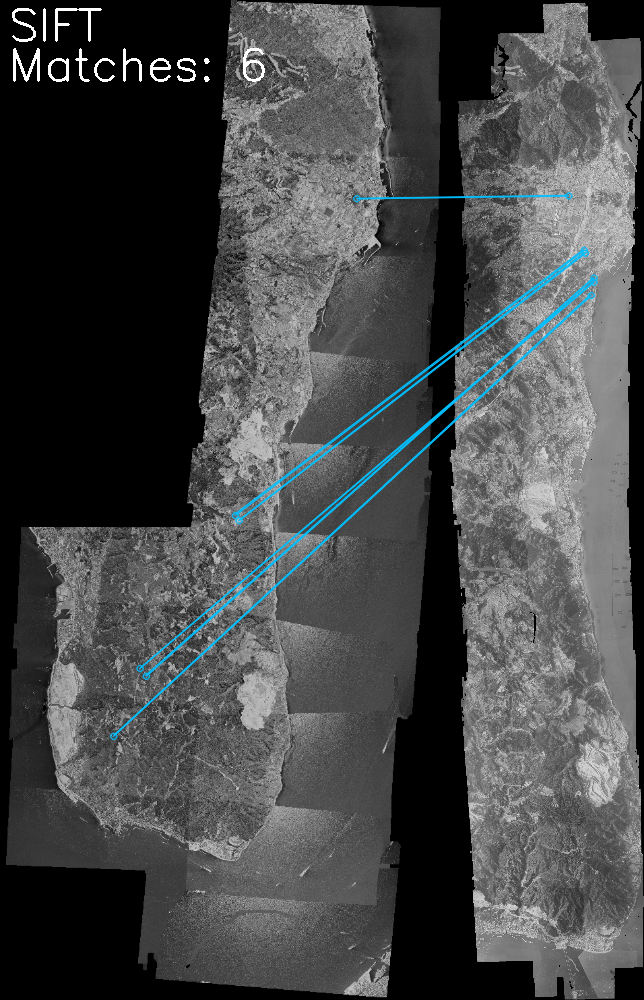
\includegraphics[width=2.6cm,angle=90]{images/Chapitre3/Homol-SIFT2Step-Rough-2DRANSAC_Ortho-MEC-Malt_Tapas_1991_Ortho-MEC-Malt_Tapas_1994.png}
			\end{minipage}%
		}
		\subfigure[$SuperGlue_{Ortho}^{RANSAC Inliers}$]{
			\begin{minipage}[t]{0.48\linewidth}
				\centering
				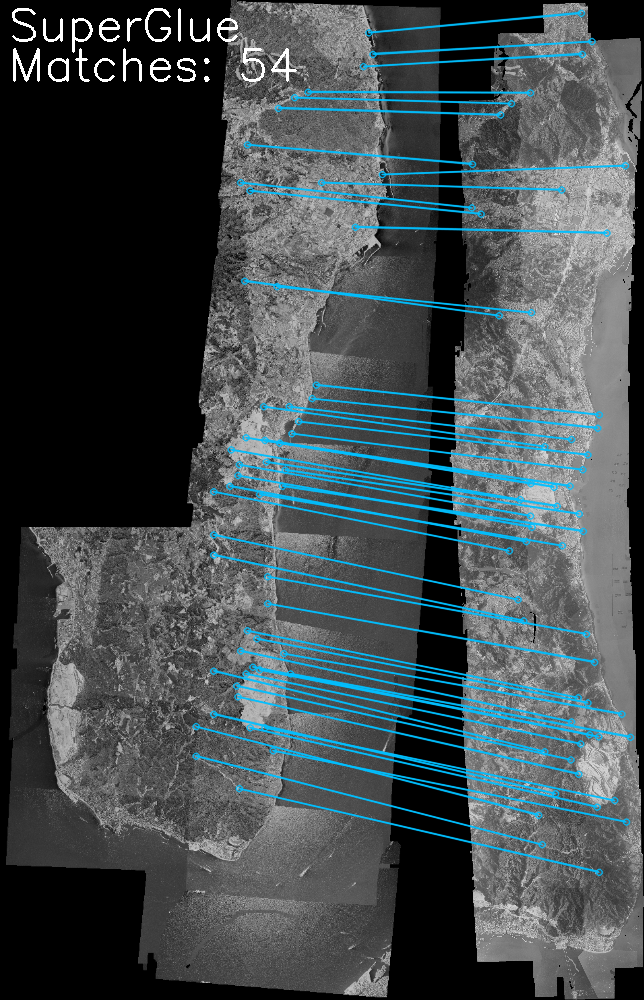
\includegraphics[width=2.6cm,angle=90]{images/Chapitre3/Homol-SubPatch-2DRANSAC_Ortho-MEC-Malt_Tapas_1991_Ortho-MEC-Malt_Tapas_1994.png}
			\end{minipage}%
		}
		%        \caption{Result of matching orthophotos (i.e. \textit{Ortho}) of Kobe 1991 and 1995. (a) Orthophotos to be matched, with red rectangles indicating the common zone. (b) Numbers of total matches and RANSAC inliers of both SIFT and SuperGlue. (c) Visualization of RANSAC inliers based on SIFT. (d) Visualization of RANSAC inliers based on SuperGlue.}
		%        \label{MatchVizKobe1991Ortho}
		%    \end{center}
		%\end{figure*} 
		%
		%\begin{figure*}[htbp]
		%    \begin{center}
		\subfigure[DSMs]{
			\begin{minipage}[t]{0.48\linewidth}
				\centering
				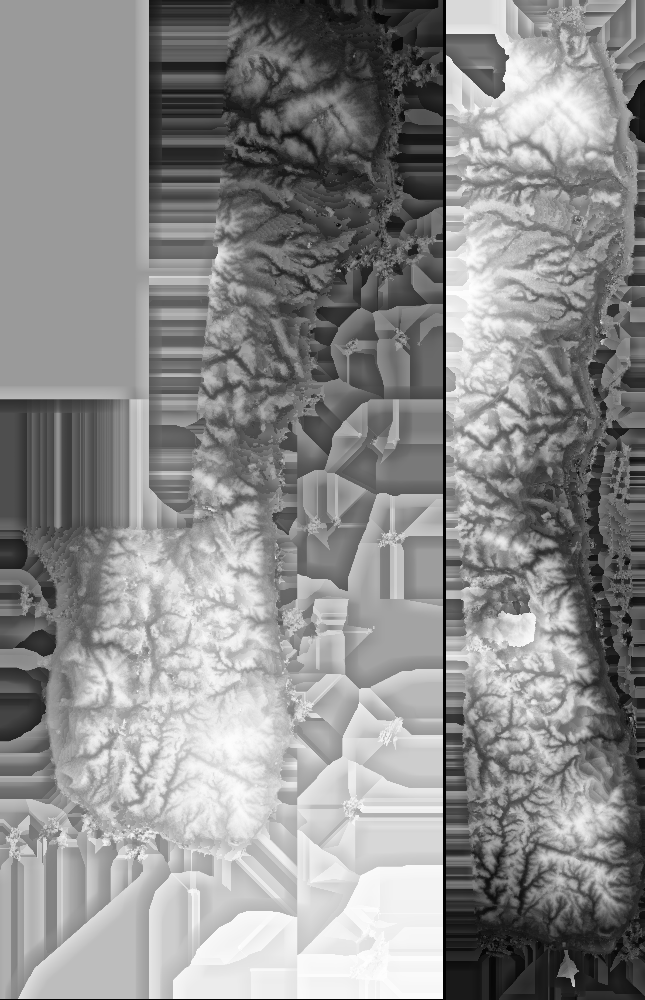
\includegraphics[width=2.3cm,angle=90]{images/Chapitre3/MEC-Malt_Tapas_1991_MEC-Malt_Tapas_1994.png}
			\end{minipage}%
		}
		\subfigure[Number of recovered matches(\textit{DSM})]{
			\begin{minipage}[t]{0.48\linewidth}
				\centering
				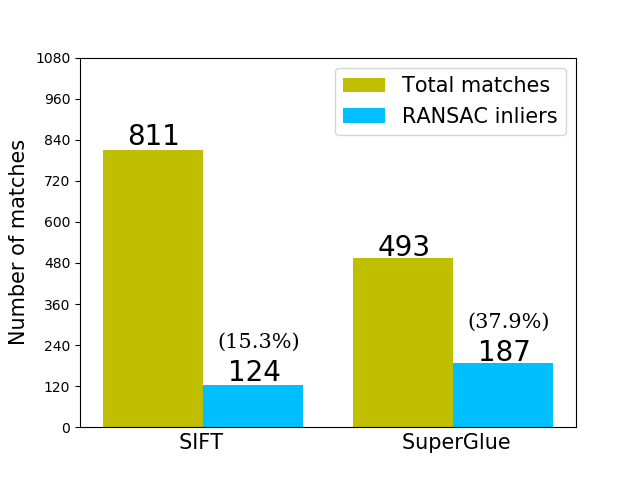
\includegraphics[width=3.5cm,trim=0 20 0 38,clip]{images/Chapitre3/PlotCurves_MEC-Malt_Tapas_1991_MEC-Malt_Tapas_1994.png}
			\end{minipage}%
		}
		\subfigure[$SIFT_{DSM}^{RANSAC Inliers}$]{
			\begin{minipage}[t]{0.48\linewidth}
				\centering
				\includegraphics[width=2.6cm,angle=90]{images/Chapitre3/Homol-SIFT2Step-Rough-2DRANSAC_MEC-Malt_Tapas_1991_MEC-Malt_Tapas_1994.png}
			\end{minipage}%
		}
		\subfigure[$SuperGlue_{DSM}^{RANSAC Inliers}$]{
			\begin{minipage}[t]{0.48\linewidth}
				\centering
				\includegraphics[width=2.6cm,angle=90]{images/Chapitre3/Homol-SubPatch-2DRANSAC_MEC-Malt_Tapas_1991_MEC-Malt_Tapas_1994.png}
			\end{minipage}%
		}
		%\caption{Result of matching DSMs (i.e. \textit{DSM}) of Kobe 1991 and 1995. (a) DSMs to be matched, with red rectangles indicating the common zone. (b) Numbers of total matches and RANSAC inliers of both SIFT and SuperGlue. (c) Visualization of RANSAC inliers based on SIFT. (d) Visualization of RANSAC inliers based on SuperGlue.}
		%\caption{{\small Result of \textit{ImgPairs}, \textit{Ortho} and \textit{DSM} on Kobe 1991 and 1995. (a, e, i) image pairs/orthophotos/DSMs to be matched, with red rectangles indicating the common zone. (b, f, j) Numbers of total matches and RANSAC inliers of both SIFT and SuperGlue on methods \textit{ImgPairs}, \textit{Ortho} and \textit{DSM} individually. (c, g, k) Visualization of RANSAC inliers based on $SIFT_{ImgPairs}$, $SIFT_{Ortho}$ and $SIFT_{DSM}$. (d, h, l) Visualization of RANSAC inliers based on $SuperGlue_{ImgPairs}$, $SuperGlue_{Ortho}$ and $SuperGlue_{DSM}$.}}
		\caption{{\scriptsize Result of \textit{ImgPairs} (a-d), \textit{Ortho} (e-h) and \textit{DSM} (i-l) on matching \textbf{Kobe 1991 and 1995}. (a, e, i) Image pairs/orthophotos/DSMs to be matched, with red rectangles indicating the common zone. (b, f, j) Numbers of total matches and RANSAC inliers of both SIFT and SuperGlue on methods \textit{ImgPairs}, \textit{Ortho} and \textit{DSM} individually. (c, g, k) Visualization of RANSAC inliers based on $SIFT_{ImgPairs}$, $SIFT_{Ortho}$ and $SIFT_{DSM}$. (d, h, l) Visualization of RANSAC inliers based on $SuperGlue_{ImgPairs}$, $SuperGlue_{Ortho}$ and $SuperGlue_{DSM}$.}}        
		\label{MatchVizKobe1991DSM}
	\end{center}
\end{figure*} 

\section{\ac{DoD}}
\label{sec:RoughDoD}
Here we display the visualization of \ac{DoD}s for dataset Pezenas and Kobe in Figure~\ref{DoDFrejus}, ~\ref{DoDPezenas} and ~\ref{DoDKobe}. The corresponding statistical information is given in Table~\ref{RoughDoDStatistic1}.\\
As can be seen, different epochs are roughly aligned with dome effect present in all the \ac{DoD}s due to poorly estimated camera parameters.\\


\begin{figure*}[htbp]
	\begin{center}
		\subfigure[\ac{DoD}$_{Pezenas1971}^{SuperGlue_{ImgPairs}}$]{
			\begin{minipage}[t]{0.31\linewidth}
				\centering
				%left, lower, right, up
				\includegraphics[width=4.2cm,trim=680 80 50 230,clip]{images/Chapitre3/DoD1971R3D-SuperGlue.png}
			\end{minipage}%
		}
		\subfigure[\ac{DoD}$_{Pezenas1971}^{SuperGlue_{Ortho}}$]{
			\begin{minipage}[t]{0.31\linewidth}
				\centering
				\includegraphics[width=4.2cm,trim=680 80 50 230,clip]{images/Chapitre3/DoD1971Ortho-SuperGlue.png}
			\end{minipage}%
		}
		\subfigure[\ac{DoD}$_{Pezenas1971}^{SuperGlue_{DSM}}$]{
			\begin{minipage}[t]{0.31\linewidth}
				\centering
				\includegraphics[width=4.2cm,trim=680 80 50 230,clip]{images/Chapitre3/DoD1971DSM-SuperGlue.png}
			\end{minipage}%
		}
		
		\subfigure[\ac{DoD}$_{Pezenas1971}^{SIFT_{ImgPairs}}$]{
			\begin{minipage}[t]{0.31\linewidth}
				\centering
				%left, lower, right, up
				\includegraphics[width=4.2cm,trim=680 80 50 230,clip]{images/Chapitre3/DoD1971R3D-SIFT.png}
			\end{minipage}%
		}
		\subfigure[\ac{DoD}$_{Pezenas1971}^{SIFT_{Ortho}}$]{
			\begin{minipage}[t]{0.31\linewidth}
				\centering
				\includegraphics[width=4.2cm,trim=680 80 50 230,clip]{images/Chapitre3/DoD1971Ortho-SIFT.png}
			\end{minipage}%
		}
		\subfigure[\ac{DoD}$_{Pezenas1971}^{SIFT_{DSM}}$]{
			\begin{minipage}[t]{0.31\linewidth}
				\centering
				\includegraphics[width=4.2cm,trim=680 80 50 230,clip]{images/Chapitre3/DoD1971DSM-SIFT.png}
			\end{minipage}%
		}
		
		\subfigure[\ac{DoD}$_{Pezenas1981}^{SuperGlue_{ImgPairs}}$]{
			\begin{minipage}[t]{0.31\linewidth}
				\centering
				%left, lower, right, up
				\includegraphics[width=4.2cm,trim=720 100 50 200,clip]{images/Chapitre3/DoD1981R3D-SuperGlue.png}
			\end{minipage}%
		}
		\subfigure[\ac{DoD}$_{Pezenas1981}^{SuperGlue_{Ortho}}$]{
			\begin{minipage}[t]{0.31\linewidth}
				\centering
				\includegraphics[width=4.2cm,trim=720 100 50 200,clip]{images/Chapitre3/DoD1981Ortho-SuperGlue.png}
			\end{minipage}%
		}
		\subfigure[\ac{DoD}$_{Pezenas1981}^{SuperGlue_{DSM}}$]{
			\begin{minipage}[t]{0.31\linewidth}
				\centering
				\includegraphics[width=4.2cm,trim=720 100 50 200,clip]{images/Chapitre3/DoD1981DSM-SuperGlue.png}
			\end{minipage}%
		}
		
		\subfigure[\ac{DoD}$_{Pezenas1981}^{SIFT_{ImgPairs}}$]{
			\begin{minipage}[t]{0.31\linewidth}
				\centering
				%left, lower, right, up
				\includegraphics[width=4.2cm,trim=720 100 50 200,clip]{images/Chapitre3/DoD1981R3D-SIFT.png}
			\end{minipage}%
		}
		\subfigure[\ac{DoD}$_{Pezenas1981}^{SIFT_{Ortho}}$]{
			\begin{minipage}[t]{0.31\linewidth}
				\centering
				\includegraphics[width=4.2cm,trim=720 100 50 200,clip]{images/Chapitre3/DoD1981Ortho-SIFT.png}
			\end{minipage}%
		}
		\subfigure[\ac{DoD}$_{Pezenas1981}^{SIFT_{DSM}}$]{
			\begin{minipage}[t]{0.31\linewidth}
				\centering
				\includegraphics[width=4.2cm,trim=720 100 50 200,clip]{images/Chapitre3/DoD1981DSM-SIFT.png}
			\end{minipage}%
		}
		\subfigure[\ac{DoD} legend]{
			\begin{minipage}[t]{1\linewidth}
				\centering
				\includegraphics[width=11cm]{images/Chapitre3/LegendDoD.png}
			\end{minipage}%
		}
		\caption{{\scriptsize \ac{DoD}s between free epoch \textbf{Pezenas 1971, 1981} and reference aerial epoch \textbf{2015} with methods $SuperGlue_{ImgPairs}$ (a, g), $SuperGlue_{Ortho}$ (b, h), $SuperGlue_{DSM}$ (c, i), $SIFT_{ImgPairs}$ (d, j), $SIFT_{Ortho}$ (e, k) and $SIFT_{DSM}$ (f, l). The prohibition sign means the corresponding method failed.}}
		\label{DoDPezenas}
	\end{center}
\end{figure*} 


\begin{figure*}[htbp]
	\begin{center}
		\subfigure[\ac{DoD}$_{Pezenas1971}^{SuperGlue_{Ortho}}$]{
			\begin{minipage}[t]{0.31\linewidth}
				\centering
				%\includegraphics[width=4.5cm,trim=680 80 50 230,clip]{images/Chapitre3/DoD1971Ortho-SuperGlue-Satellite.png}
				\includegraphics[width=2cm]{images/Chapitre3/NoDoD.png}
			\end{minipage}%
		}
		\subfigure[\ac{DoD}$_{Pezenas1971}^{SuperGlue_{DSM}}$]{
			\begin{minipage}[t]{0.31\linewidth}
				\centering
				\includegraphics[width=4.5cm,trim=680 80 50 230,clip]{images/Chapitre3/DoD1971DSM-SuperGlue-Satellite.png}
			\end{minipage}%
		}\\
		
		\subfigure[\ac{DoD}$_{Pezenas1971}^{SIFT_{Ortho}}$]{
			\begin{minipage}[t]{0.31\linewidth}
				\centering
				\includegraphics[width=2cm]{images/Chapitre3/NoDoD.png}
			\end{minipage}%
		}
		\subfigure[\ac{DoD}$_{Pezenas1971}^{SIFT_{DSM}}$]{
			\begin{minipage}[t]{0.31\linewidth}
				\centering
				\includegraphics[width=4.2cm,trim=720 100 50 200,clip]{images/Chapitre3/DoD1971DSM-SIFT-Satellite.png}
			\end{minipage}%
		}\\
		
		\subfigure[\ac{DoD}$_{Pezenas1981}^{SuperGlue_{Ortho}}$]{
			\begin{minipage}[t]{0.31\linewidth}
				\centering
				\includegraphics[width=4.2cm,trim=900 100 250 200,clip]{images/Chapitre3/DoD1981Ortho-SuperGlue-Satellite.png}
			\end{minipage}%
		}
		\subfigure[\ac{DoD}$_{Pezenas1981}^{SuperGlue_{DSM}}$]{
			\begin{minipage}[t]{0.31\linewidth}
				\centering
				\includegraphics[width=4.2cm,trim=900 100 250 200,clip]{images/Chapitre3/DoD1981DSM-SuperGlue-Satellite.png}
			\end{minipage}%
		}\\
		
		
		\subfigure[\ac{DoD}$_{Pezenas1981}^{SIFT_{Ortho}}$]{
			\begin{minipage}[t]{0.31\linewidth}
				\centering
				\includegraphics[width=2cm]{images/Chapitre3/NoDoD.png}
			\end{minipage}%
		}
		\subfigure[\ac{DoD}$_{Pezenas1981}^{SIFT_{DSM}}$]{
			\begin{minipage}[t]{0.31\linewidth}
				\centering
				\includegraphics[width=4.2cm,trim=900 100 250 200,clip]{images/Chapitre3/DoD1981DSM-SIFT-Satellite.png}
			\end{minipage}%
		}\\
		
		
		\subfigure[\ac{DoD} legend]{
			\begin{minipage}[t]{1\linewidth}
				\centering
				\includegraphics[width=11cm]{images/Chapitre3/LegendDoD.png}
			\end{minipage}%
		}
		\caption{{\scriptsize \ac{DoD}s between free epoch \textbf{Pezenas 1971, 1981} and reference satellite epoch \textbf{2014} with methods $SuperGlue_{Ortho}$ (a, e), $SuperGlue_{DSM}$ (b, f), $SIFT_{Ortho}$ (c, g) and $SIFT_{DSM}$ (d, h). The holes among them are areas covered with clouds which are masked out. The prohibition sign means the corresponding method failed.}}
		\label{DoDPezenas-Satellite}
	\end{center}
\end{figure*} 


\begin{figure*}[htbp]
	\begin{center}
		\subfigure[\ac{DoD}$_{Kobe}^{SuperGlue_{ImgPairs}}$]{
			\begin{minipage}[t]{1\linewidth}
				\centering
				%left, lower, right, up
				\includegraphics[width=12cm,trim=700 450 180 560,clip]{images/Chapitre3/DoD1991R3D-SuperGlue.png}
			\end{minipage}%
		}
		\subfigure[\ac{DoD}$_{Kobe}^{SuperGlue_{Ortho}}$]{
			\begin{minipage}[t]{1\linewidth}
				\centering
				\includegraphics[width=12cm,trim=700 450 180 560,clip]{images/Chapitre3/DoD1991Ortho-SuperGlue.png}
			\end{minipage}%
		}
		\subfigure[\ac{DoD}$_{Kobe}^{SuperGlue_{DSM}}$]{
			\begin{minipage}[t]{1\linewidth}
				\centering
				\includegraphics[width=12cm,trim=700 450 180 560,clip]{images/Chapitre3/DoD1991DSM-SuperGlue.png}
			\end{minipage}%
		}
		
		\subfigure[\ac{DoD}$_{Kobe}^{SIFT_{ImgPairs}}$]{
			\begin{minipage}[t]{1\linewidth}
				\centering
				%left, lower, right, up
				\includegraphics[width=2cm]{images/Chapitre3/NoDoD.png}
			\end{minipage}%
		}
		\subfigure[\ac{DoD}$_{Kobe}^{SIFT_{Ortho}}$]{
			\begin{minipage}[t]{1\linewidth}
				\centering
				\includegraphics[width=2cm]{images/Chapitre3/NoDoD.png}
			\end{minipage}%
		}
		\subfigure[\ac{DoD}$_{Kobe}^{SIFT_{DSM}}$]{
			\begin{minipage}[t]{1\linewidth}
				\centering
				\includegraphics[width=12cm,trim=700 450 180 560,clip]{images/Chapitre3/DoD1991DSM-SIFT.png}
			\end{minipage}%
		}
		
		\subfigure[\ac{DoD} legend]{
			\begin{minipage}[t]{1\linewidth}
				\centering
				\includegraphics[width=11cm]{images/Chapitre3/LegendDoD.png}
			\end{minipage}%
		}
		\caption{{\scriptsize \ac{DoD}s between free epoch \textbf{Kobe 1991} and reference epoch \textbf{1995} with methods $SuperGlue_{ImgPairs}$ (a), $SuperGlue_{Ortho}$ (b), $SuperGlue_{DSM}$ (c), $SIFT_{ImgPairs}$ (d), $SIFT_{Ortho}$ (e) and $SIFT_{DSM}$ (f). The prohibition sign means the corresponding method failed.}}
		\label{DoDKobe}
	\end{center}
\end{figure*} 

\begin{table}%[H]
	\footnotesize
	\centering
	\begin{tabular}{||l|l|c|c|c||}\hline
		& &$\mu$ [m]&$\sigma$ [m]&$|\mu|$ [m]\\\hline\hline		
		\multirow{6}{*}{$DoD^{Pezenas}_{1971-2015}$}
		&${SuperGlue_{ImgPairs}}$ & -7.42 & 16.60 & 13.78\\
		&${SuperGlue_{Ortho}}$ & -8.46 & 22.36 & 16.68\\
		&${SuperGlue_{DSM}}$ & 4.71 & 16.85 & 14.20\\
		&${SIFT_{ImgPairs}}$ & 2.77 & 16.58 & 13.98\\
		&${SIFT_{Ortho}}$ & -8.05 & 21.71 & 17.07\\
		&${SIFT_{DSM}}$ & -0.75 & 17.75 & \textbf{13.74}\\\hline
		
		\multirow{6}{*}{$DoD^{Pezenas}_{1981-2015}$}
		&${SuperGlue_{ImgPairs}}$ & -0.39 & 9.12 & \textbf{7.10}\\
		&${SuperGlue_{Ortho}}$ & -2.60 & 9.93 & 7.76\\
		&${SuperGlue_{DSM}}$ & 0.64 & 9.15 & 7.24\\
		&${SIFT_{ImgPairs}}$ & -2.01 & 10.07 & 7.80\\
		&${SIFT_{Ortho}}$ & -4.80 & 13.25 & 10.33\\
		&${SIFT_{DSM}}$ & -0.73 & 9.67 & 7.42\\\hline
		
		%%%%%%%%%%%%%%%%%%%%%%%%satellite
		\multirow{4}{*}{$DoD^{Pezenas}_{1971-2014(Satellite)}$}
		&${SuperGlue_{Ortho}}$ & / & / & /\\
		&${SuperGlue_{DSM}}$ & -3.70 & 10.65 & 8.29\\
		%&${SuperGlue_{DSM}}$ & -1.85 & 13.24 & 9.15\\
		&${SIFT_{Ortho}}$ & / & / & /\\
		&${SIFT_{DSM}}$ & -0.68 & 8.11 & \textbf{5.80} \\\hline
		%&${SIFT_{DSM}}$ & 0.58 & 7.82 & \textbf{3.18}\\\hline
		
		\multirow{4}{*}{$DoD^{Pezenas}_{1981-2014(Satellite)}$}
		&${SuperGlue_{Ortho}}$ & -0.64 & 6.18 & 4.48\\
		%&${SuperGlue_{Ortho}}$ & 0.59 & 9.87 & 5.66\\
		&${SuperGlue_{DSM}}$ & -1.15 & 6.07 & 4.55\\
		%&${SuperGlue_{DSM}}$ & 0.31 & 9.88 & 5.73\\
		&${SIFT_{Ortho}}$ & / & / & /\\
		&${SIFT_{DSM}}$ & -1.41 & 6.14 & \textbf{4.45} \\\hline
		%&${SIFT_{DSM}}$ & 0.46 & 5.96 & \textbf{1.92}\\\hline
		
		
		\multirow{6}{*}{$DoD^{Kobe}_{1991-1995}$}
		&${SuperGlue_{ImgPairs}}$ & -1.63 & 13.85 & \textbf{7.24}\\
		%&${SIFT_{ImgPairs}}$ & 167.46 & 121.26 & 168.47\\
		&${SuperGlue_{Ortho}}$ & -0.54 & 14.83 & 7.78\\
		%&${SIFT_{Ortho}}$ & 4.29 & 41.89 & 26.01\\
		&${SuperGlue_{DSM}}$ & -0.75 & 14.62 & 7.95\\
		&${SIFT_{ImgPairs}}$ & / & / & / \\
		&${SIFT_{Ortho}}$ & / & / & / \\
		&${SIFT_{DSM}}$ & 0.27 & 14.40 & 7.57\\\hline
		
	\end{tabular}
	\caption{Average value $\mu$, standard deviation $\sigma$, and absolute average value $|\mu|$ of all the \ac{DoD}s in Figure~\ref{DoDPezenas}, ~\ref{DoDPezenas-Satellite} and ~\ref{DoDKobe}.}
	\label{RoughDoDStatistic1}
\end{table}
